%  LaTeX support: latex@mdpi.com
%=================================================================
% Fix for older pdfTeX / xcolor incompatibility
% \PassOptionsToPackage{dvips}{xcolor}  % removed: conflicts with pdftex driver
\documentclass[fire,article,submit,pdftex]{../Definitions/mdpi}

% Additional packages
% ---------------------------------------------------------------
% SUBMISSION CHECKLIST (v10 updates):
% 1. Rename all main figure files to match final paper numbering:
%    Figure_0_timeline -> Figure_1, Figure_1_framework -> Figure_2,
%    Figure_2_reliability -> Figure_3, Figure_3_calibration -> Figure_4,
%    Figure_4_ablation -> Figure_5 (paper auto-numbers as Figure 6),
%    Figure_5_bootstrap -> Figure_6 (paper: Figure 7),
%    Figure_6_distributions -> Figure_7 (paper: Figure 8),
%    Figure_7_baselines -> Figure_8 (paper: Figure 5),
%    Figure_8_recalibration -> Figure_9 (paper: Figure 9).
%    Note: baseline (Figure_7_baselines) appears BEFORE ablation
%    (Figure_4_ablation) in the paper, so paper numbering is:
%    Fig5=baselines, Fig6=ablation.
% 2. [Removed: Figure S2 (outer-fold prediction distributions) deleted from paper.]
% 3. Verify Graphical Abstract numbers match final paper values
%    (24h terciles: 0.0% / 4.5% / 92.3% per Table 6).
% ---------------------------------------------------------------
\usepackage[utf8]{inputenc}
\usepackage{graphicx}
\setlength{\headheight}{20.0pt}
\addtolength{\topmargin}{-8.0pt}
\usepackage{amsmath,amssymb}
% Prevent widow/orphan lines and improve float placement
\widowpenalty=10000
\clubpenalty=10000
\brokenpenalty=4991
% Unicode characters that may appear in SVG text layers
\DeclareUnicodeCharacter{2264}{$\leq$}%   ≤
\DeclareUnicodeCharacter{2265}{$\geq$}%   ≥
\DeclareUnicodeCharacter{2212}{$-$}%      − (minus sign)
\DeclareUnicodeCharacter{00D7}{$\times$}% ×
\DeclareUnicodeCharacter{03B1}{$\alpha$}% α
\DeclareUnicodeCharacter{03B2}{$\beta$}%  β
\usepackage{booktabs}
\usepackage{multirow}
\usepackage{siunitx}
\usepackage{algorithmic}
\usepackage{algorithm}

% Pagination and metadata
\firstpage{1}
\makeatletter
\setcounter{page}{\@firstpage}
\makeatother
\pubvolume{1}
\issuenum{1}
\articlenumber{0}
\pubyear{2026}
\copyrightyear{2026}
\datereceived{ }
\daterevised{ }
\dateaccepted{ }
\datepublished{ }

%=================================================================
\Title{A Survival--Probability Fusion Prototype for Censor-Aware Multi-Horizon Wildfire Threat Forecasting and Decision-Utility Evaluation}

\Author{Zhengyang Ren $^{1,*}$}
\AuthorNames{Zhengyang Ren}

\address{%
$^{1}$ \quad Jiaying University, 100 Meisong Road, Meijiang District, Meizhou 514015, Guangdong, China; d58350215@gmail.com}

\corres{Correspondence: d58350215@gmail.com}

%=================================================================
\abstract{%
Wildfire evacuation planning requires calibrated, multi-horizon threat-time probabilities, yet existing prediction approaches rarely handle right censoring, cross-horizon coherence, and probability calibration within a single pipeline.
We propose a survival--probability fusion framework that integrates an XGBoost accelerated failure time backbone, horizon-specific probability heads, post-hoc beta calibration, and monotone-constrained fusion to produce coherent 12, 24, and 48~h threat probabilities.
The framework was evaluated on 221 wildfire--zone encounters (69 events, 152 censored; WiDS Datathon 2026) using nested five-fold cross-validation with inner cross-fitting.
The full model achieved Uno's IPCW C-index of 0.941 (95\% bootstrap CI 0.924--0.959) and a mean Brier score of 0.041.
Monotone fusion corrected logically incoherent probability sequences in 24.9\% of observations at the 24--48~h transition.
Risk stratification at 24~h separated observed event rates into 0.0\%, 4.5\%, and 92.3\% across predicted terciles.
A Random Survival Forest and lean AFT-centred variants matched or exceeded the full architecture on aggregate metrics, indicating that at the present sample size (events-per-variable $\approx$ 2.0), the framework's value is primarily structural rather than performance-based.
Formal incident-grouped and external spatiotemporal validation remain necessary before operational deployment.
}

\keyword{wildfire forecasting; evacuation risk; survival analysis; censoring; multi-horizon prediction; calibration; risk stratification; monotone fusion; decision curve analysis}

%%%%%%%%%%%%%%%%%%%%%%%%%%%%%%%%%%%%%%%%%%
\begin{document}
%%%%%%%%%%%%%%%%%%%%%%%%%%%%%%%%%%%%%%%%%%

\section{Introduction}\label{sec:introduction}

Wildfire risk management increasingly requires not merely a binary ``will fire arrive'' prediction but a probabilistic estimate of \emph{when} a fire will threaten a given evacuation zone.
Horizon-specific threat probabilities directly inform pre-evacuation readiness: emergency managers must rank simultaneously threatened zones by time-criticality, stage resources ahead of a fire front, and trigger zone-level alerts with sufficient lead time~\cite{Finney2001,Xi2019,Stephens2018}.
With the frequency, intensity, and spatial extent of large wildfires rising over the past two decades~\cite{Jain2022,Cunningham2024,Turco2023,Luo2024,Jones2022,Kolden2024,Higuera2021}, the demand for calibrated, multi-horizon decision-support tools that go beyond distance-based heuristics has grown correspondingly~\cite{Radeloff2023,Tonini2020}.

Existing approaches to wildfire threat prediction can be broadly grouped into three categories.
First, physics-informed estimated-time-of-arrival (ETA) models compute arrival times from distance and fire-spread rate~\cite{Finney2001,Cruz2003}, but produce point estimates rather than probabilistic outputs and cannot naturally handle right-censored observations, which arise when monitoring ends before fire arrival.
Second, single-horizon machine learning classifiers predict a binary outcome at a fixed time window, discarding information from censored cases and failing to ensure probability consistency across multiple windows~\cite{Jaafari2019,Gigovic2019,Chen2024wui}.
Third, survival analysis approaches---such as Cox proportional-hazards or accelerated failure time (AFT) models---natively handle censoring and produce survival curves from which horizon-specific cumulative incidence probabilities $P(T \leq h)$ can be derived; these probabilities are inherently monotone non-decreasing by construction~\cite{Wiegrebe2024,Taylor2013}.
However, when \emph{separate} horizon-specific classifiers are trained independently, the resulting probability estimates are not guaranteed to be mutually consistent across horizons, and the survival-derived probabilities may require post-hoc calibration to align with observed event rates at each discrete horizon~\cite{VanCalster2019}.

Three methodological gaps remain.
First, right-censored observations are common in wildfire encounter datasets; ignoring them introduces survivorship bias, and the modest sample sizes typical of labelled wildfire records further demand rigorous cross-validation and regularisation~\cite{Steyerberg2019,Collins2024,Riley2020}.
Second, operational decision-support requires probability estimates at multiple discrete horizons (e.g., 12, 24, 48~h) that are monotonically non-decreasing ($P(T \leq 12) \leq P(T \leq 24) \leq P(T \leq 48)$) to remain logically coherent.
Third, discrimination alone is insufficient for threshold-based evacuation triggers; absolute probability calibration is necessary for zone-level decision rules to be actionable~\cite{VanCalster2019}.

In this study, we present a survival--probability fusion framework designed to address these gaps within an internally validated decision-support prototype.
Given the modest sample size (221 observations, 69 events), the framework is positioned as a methodological contribution rather than a claim of performance superiority.
The contributions are threefold:
\begin{enumerate}
    \item A censor-aware multi-horizon prediction framework unifying an AFT survival backbone with horizon-targeted probability heads, post-hoc calibration, and monotone-constrained fusion to produce coherent threat-time probabilities at 12, 24, and 48~h---with empirical evidence that explicit monotone enforcement corrects logically incoherent probability sequences in approximately 25\% of observations at the 24--48~h transition;
    \item A leakage-controlled nested cross-validation protocol with inner cross-fitting that prevents information contamination between meta-feature generation and fusion weight estimation;
    \item A transparent evaluation with systematic ablation, baseline comparisons against both survival and non-survival alternatives, and decision curve analysis---including candid reporting of cases where simpler baselines matched or exceeded the full framework.
\end{enumerate}

\section{Materials and Methods}\label{sec:methods}

\subsection{Study Design and Data Source}\label{sec:data}

This is a retrospective predictive modelling study.
The dataset was obtained from the WiDS Datathon 2026 wildfire prediction competition and contains records derived from real wildfire events in the western United States.
Each observation represents a single \emph{fire--zone pair}: one wildfire event paired with one evacuation zone, characterised by spatio-temporal and dynamic fire-behaviour variables computed from fire perimeter data observed during the first five hours after ignition.
The analysis unit throughout this study is the fire--zone pair; each such pair contributes exactly one observation.
The labelled training set comprises 221 fire--zone pairs across 37 variables, with 69 events (fire entering within 5~km of the evacuation-zone centroid) and 152 right-censored observations (monitoring ended before fire arrival or the fire was contained).
A held-out test set of 95 observations (35 variables) was available but lacked outcome labels; all model development and evaluation were therefore conducted exclusively using the 221-observation training set under nested cross-validation.
All predictor variables were available at or before the end of the five-hour observation window, ensuring no information leakage from the future.

\subsection{Outcome Definition and Censoring}\label{sec:outcome}

The primary outcome is the time from the end of the initial five-hour observation window to the fire perimeter entering within 5~km of the evacuation-zone centroid, measured in hours.
This definition follows the WiDS Datathon 2026 task specification: features are derived from fire behaviour observed during the first five hours after ignition, and the prediction target is whether the fire enters a 5~km radius around the zone centroid within 12, 24, or 48~h of the observation window endpoint (Figure~\ref{fig:timeline}).
Right censoring occurs when monitoring ends (e.g., fire is contained, observation period lapses) before the fire reaches the 5~km threshold.
Notably, censoring from fire containment may not be fully non-informative: containment is an intervention correlated with fire behaviour covariates rather than a random process, departing from the standard independent right-censoring assumption~\cite{Steyerberg2019}.

\begin{figure}[!ht]
\centering
    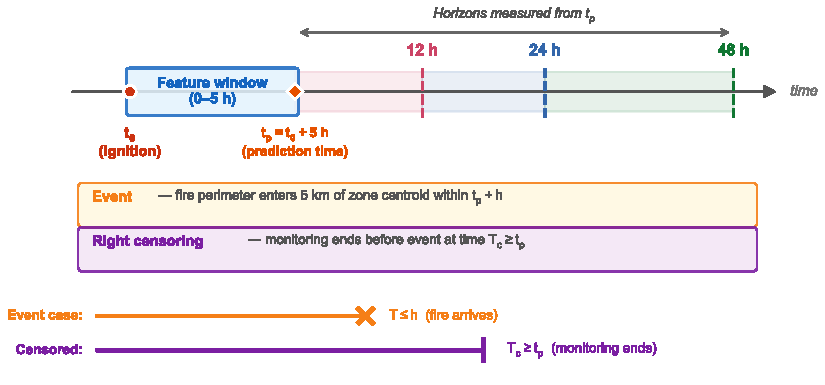
\includegraphics[width=\linewidth]{figures/main/Figure_1_prediction_timeline.pdf}
\caption{Prediction timeline. Features are extracted from the first five hours after ignition ($t_0$). The prediction time $t_p = t_0 + 5$~h defines the origin for all horizons. The event is defined as the fire perimeter entering within 5~km of the evacuation-zone centroid. Observations are right-censored if monitoring ends before the event occurs. An ``$\times$'' denotes an observed event (fire arrival within the horizon); a vertical bar ``$|$'' denotes right censoring (monitoring terminated before the event).}\label{fig:timeline}
\end{figure}

Three main prediction horizons---12~h, 24~h, and 48~h---were selected to span the operationally relevant window for evacuation planning: 12~h represents a critical near-term alert threshold, 24~h corresponds to a standard pre-evacuation preparation period, and 48~h supports medium-range resource positioning~\cite{Stephens2018,Taylor2013}.
An additional 72~h horizon was computed but yielded a degenerate positive rate of 100\% (all eligible observations experienced the event), rendering it uninformative; results for 72~h are therefore confined to Supplementary Materials (Table~S1).

Censor-aware binary targets for each horizon $h$ were defined as follows.
An observation is \emph{eligible} at horizon $h$ if either an event occurred at any time or censoring occurred at a time $\geq h$.
Among eligible observations, the target $Y_h = 1$ if the event occurred at time $T \leq h$, and $Y_h = 0$ otherwise.
This definition correctly excludes observations that were censored before horizon $h$ and whose true status at $h$ is unknown.
This binary formulation does not distinguish between narrowly missed events (e.g., fire arriving at $T$ just beyond $h$) and clearly non-threatened observations; a continuous-time competing-risks formulation could address this distinction in future work.
The eligible sample sizes and positive rates at each horizon are reported in Table~\ref{tab:horizons}.

\begin{table}[!ht]
\caption{Censor-aware target characteristics for each prediction horizon.}\label{tab:horizons}
\begin{tabular}{lccc}
\toprule
\textbf{Horizon} & \textbf{Eligible $n$} & \textbf{Positives} & \textbf{Positive Rate (\%)} \\
\midrule
12~h  & 215 & 49  & 22.8 \\
24~h  & 196 & 63  & 32.1 \\
48~h  & 166 & 66  & 39.8 \\
72~h$^\dagger$ & 69  & 69  & 100.0 \\
\bottomrule
\multicolumn{4}{l}{\footnotesize $^\dagger$Degenerate; confined to Supplementary Materials.}
\end{tabular}
\end{table}

\subsection{Predictors and Feature Engineering}\label{sec:features}

Input features were organised into four conceptual groups:

\paragraph{Distance and urgency features.}
Raw distance to the closest fire perimeter was transformed into log-distance ($\log(1 + d)$), inverse distance ($1 / (1000 + d)$), and a short-range urgency score ($\exp(-d / 2500)$).
An estimated time of arrival (ETA) was computed as $\text{ETA} = d / \max(v_{\mathrm{closing}}, 50)$, clipped at 240~h.

\paragraph{Speed and alignment features.}
Closing speed (signed and absolute), centroid speed, and an alignment measure capturing the angular correspondence between fire spread direction and the vector toward the zone boundary were retained.
A directional push interaction was computed as $\max(v_{\mathrm{closing}}, 0) \times |\text{alignment}|$.

\paragraph{Growth and spread dynamics.}
Features included area growth rate (ha/h), radial growth rate (m/h), log-transformed growth ($\log(1 + \text{growth})$), and two interaction terms: closing speed $\times$ log-growth and area growth rate $\times$ alignment.

\paragraph{Temporal and regime features.}
Cyclical encoding (sine/cosine) was applied to event start hour (period = 24), day of week (period = 7), and month (period = 12).
Three binary regime indicators were defined based on distance thresholds: \emph{threat} ($d < 4500$~m), \emph{boundary} ($4500 \leq d \leq 7000$~m), and \emph{far} ($d > 7000$~m).
These thresholds were chosen as pragmatic operational cutoffs informed by general fire-management considerations: 4500~m is within the range at which ember transport and spot-fire ignition have been reported to pose structural threat under moderate-to-high wind conditions in coniferous fuel types~\cite{Cruz2003,Finney2001}, while 7000~m is broadly consistent with outer perimeters used for pre-evacuation staging areas in California wildfire management~\cite{Dolan2022}; however, these values should be regarded as engineering heuristics rather than established domain consensus, and their appropriateness may vary across fuel types and terrain.
The ETA computation clipped closing speed at a minimum of 50~m/h (a conservative lower bound for slow-moving ground fires) and capped the estimated arrival time at 240~h (10~days), beyond which the prediction is operationally uninformative~\cite{Taylor2013}.

In total, the full feature set comprised 26 engineered features plus 8 retained original dataset columns (after deduplication and exclusion of identifier and outcome variables), yielding 34 features available for modelling (see Supplementary Table~S0 for the complete feature dictionary).
Missing values were imputed using median substitution for continuous predictors and mode substitution for binary indicators, applied within each outer training fold to prevent leakage; in practice, no variables in the analysis dataset contained missing values (Supplementary Table~S11), so the imputation step served as a precautionary safeguard rather than correcting actual missingness.
A ``thin'' feature subset restricted to the 26 engineered features was also evaluated in the ablation study to assess the contribution of original dataset columns.

\subsection{Proposed Framework}\label{sec:model}

The proposed framework consists of four modules (Figure~\ref{fig:framework}):

\begin{figure}[!ht]
\begin{adjustwidth}{-\extralength}{0cm}
    \centering
    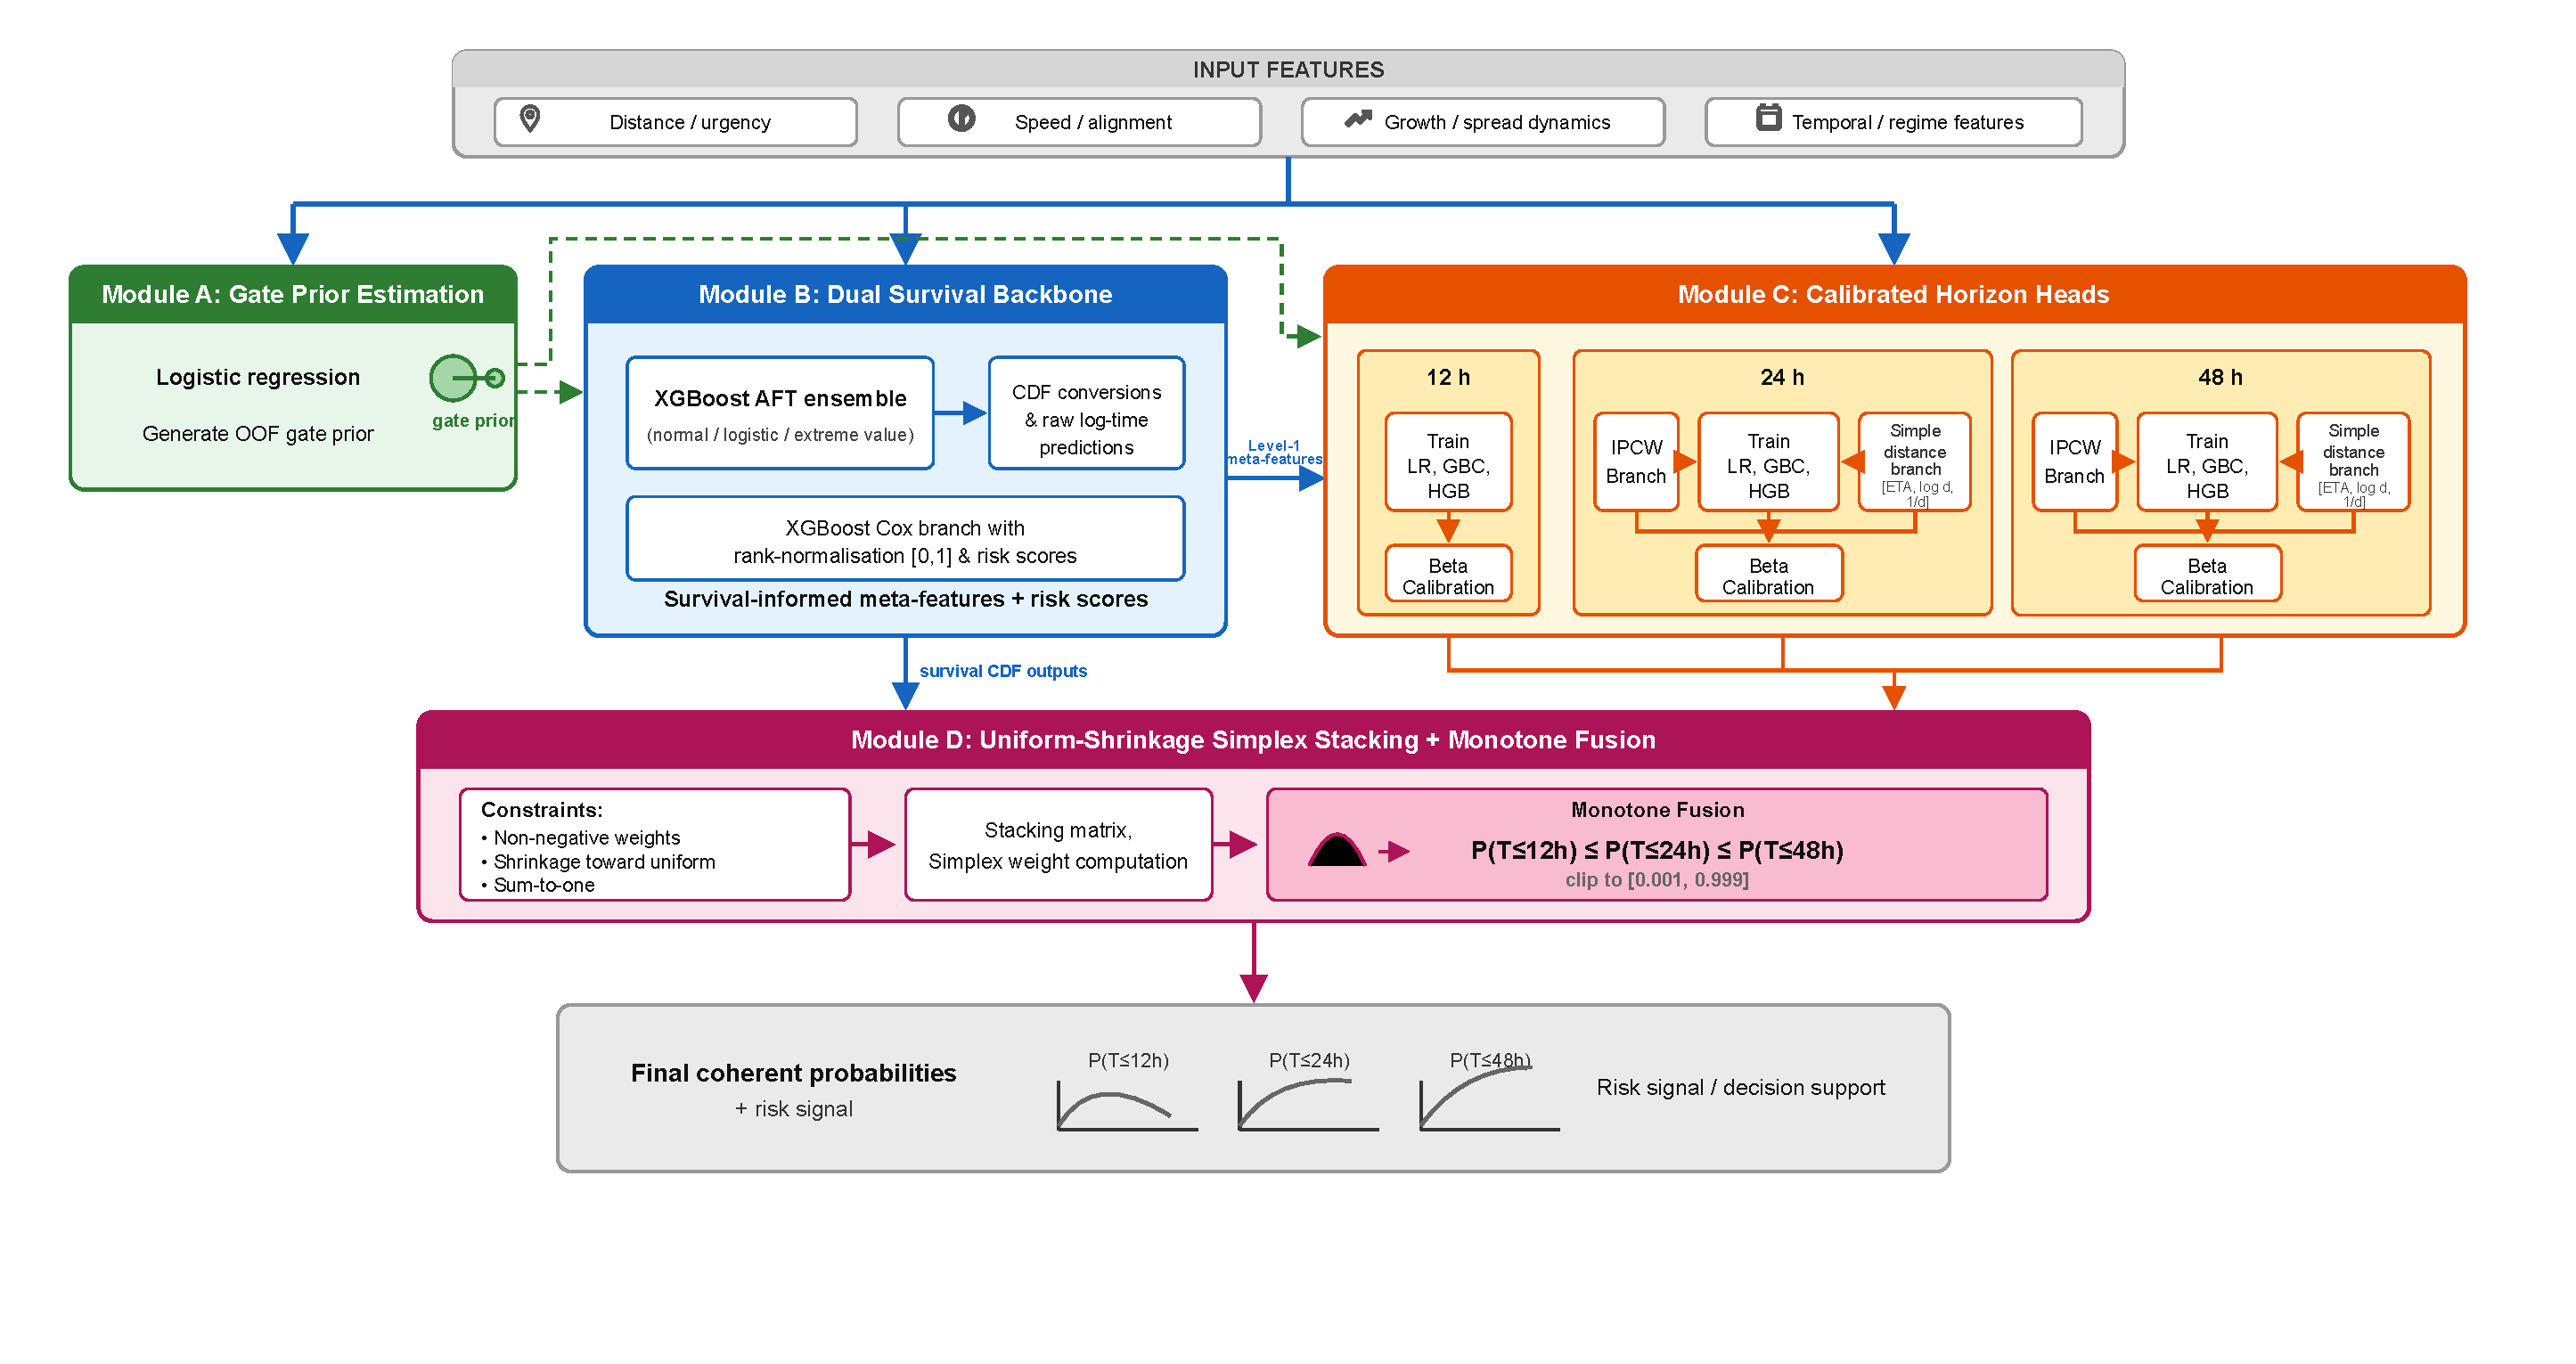
\includegraphics[width=\linewidth]{figures/main/Figure_2_framework_schematic.pdf}
\end{adjustwidth}
    \caption{Framework schematic. Module~A estimates a gate prior via logistic regression. Module~B comprises a dual survival backbone (XGBoost AFT and Cox proportional hazards). Module~C trains calibrated direct probability heads (logistic regression, gradient boosting, histogram gradient boosting with beta calibration) at each horizon. Module~D performs uniform-shrinkage simplex stacking followed by monotone-constrained fusion to produce final coherent probabilities $P(T \leq h)$ for $h \in \{12, 24, 48\}$.}\label{fig:framework}
\end{figure}

\subsubsection{Module A: Gate Prior Estimation}

A logistic regression model is trained on the full feature set to predict a binary event indicator.
The resulting out-of-fold (OOF) predicted probabilities serve as a \emph{gate prior}---a soft signal capturing the baseline likelihood that a fire will reach the zone---which is injected as an additional feature into Modules~B and C.
This data-driven summary reduces redundancy among raw features, functioning as a stacking-level shrinkage signal.

\subsubsection{Module B: Dual Survival Backbone}

Two complementary survival models are trained:

\emph{XGBoost AFT ensemble.}
Three XGBoost~\cite{Chen2016} AFT models with different distributional assumptions (normal, logistic, extreme value) and hyperparameter settings are fitted.
For each observation, the predicted log-survival time from each AFT model is converted to a horizon-specific probability via the corresponding distributional CDF.
The ensemble of AFT-derived probabilities, along with the raw log-time predictions, forms a set of survival-informed meta-features.

\emph{Cox proportional-hazards ranking branch.}
Three XGBoost Cox models with varying depth and learning rate configurations are fitted to the same features.
The predicted risk scores provide a discrimination-focused signal that complements the AFT branch's emphasis on probability estimation.
Risk scores are rank-normalised to the $[0, 1]$ interval before entering the stacking matrix.

Both branches are trained exclusively on inner-fold data with OOF predictions generated via cross-fitting, ensuring that no observation's meta-features depend on a model that saw the same observation during training.

\emph{Design note on the Cox branch's role.}
The Cox branch contributes exclusively to the composite ranking signal used for discrimination analysis and is \emph{not} injected into the horizon-wise probability stacking matrix in Module~D.
Consequently, adding or removing the Cox branch may change the concordance index (discrimination) but leaves Brier scores, ECE, and calibration slopes unchanged.
This separation is by design: the Cox branch serves as a ranking enhancer, not a calibration source.

\subsubsection{Module C: Calibrated Horizon Heads}

For each horizon $h \in \{12, 24, 48\}$, three direct classifiers---logistic regression (LR), gradient boosting classifier (GBC), and histogram gradient boosting classifier (HGB)---are trained on the censor-aware binary target $Y_h$.
The input feature vector includes all Level~1 meta-features from Modules~A and B, alongside the original engineered features.
Beta calibration~\cite{Kull2017} (three-parameter form) is applied post-hoc to each classifier's OOF probability outputs to improve probability reliability; calibration parameters are estimated on the inner-fold OOF predictions and applied to outer-fold predictions.
However, the three-parameter beta calibration may itself be susceptible to overfitting when the effective eligible sample within each inner fold is small (e.g., $\sim$35 eligible observations at some horizons); a two-parameter or simpler isotonic alternative may prove more stable in future work.

Additionally, at 24~h and 48~h, two supplementary branches are optionally included:
(i)~an inverse-probability-of-censoring-weighted (IPCW) branch using LightGBM classifiers, which assigns each observation a weight $w_i = \delta_i / \hat{G}(T_i)$, where $\delta_i$ is the event indicator and $\hat{G}(T_i)$ is the Kaplan--Meier estimate of the censoring survival function evaluated at the observed time~\cite{Uno2011,Graf1999}; censored observations receive zero weight and thus do not contribute to the IPCW loss, consistent with the standard formulation; and
(ii)~a simple distance-based branch comprising a logistic regression on the $[\text{ETA}, \log d, 1/d]$ feature triple, providing a physics-informed anchor.

\subsubsection{Module D: Uniform-Shrinkage Simplex Stacking and Monotone Fusion}

All horizon-specific probability estimates from Module~C (and from the survival CDF conversions in Module~B) are collected into a stacking matrix~\cite{Wolpert1992,VanderLaan2007}.
Fusion weights are learned by minimising the Brier score~\cite{Brier1950} on the inner OOF set, subject to non-negativity constraints and regularised toward the uniform distribution (Equation~\eqref{eq:stacking}):
\begin{equation}
    \mathbf{w}^* = \arg\min_{\mathbf{w} \geq 0} \left[ \frac{1}{n} \sum_{i=1}^{n} \left( y_i - \mathbf{w}^\top \mathbf{s}_i \right)^2 + \lambda \left\| \mathbf{w} - \frac{1}{K}\mathbf{1} \right\|_2^2 \right],
    \label{eq:stacking}
\end{equation}
where $\mathbf{s}_i$ is the vector of stacked probability estimates for observation $i$, $K$ is the number of base learners, and $\lambda = 1.0$ is a fixed regularisation hyperparameter (not tuned on data) controlling the strength of shrinkage toward the uniform prior.
The value $\lambda = 1.0$ was chosen to impose moderate regularisation: it balances the data-driven Brier loss (whose magnitude is $O(10^{-2})$ per observation) against a meaningful pull toward equal weighting, thereby discouraging dominance by any single base learner without suppressing informative weight differentiation entirely.
A sensitivity analysis over $\lambda \in \{0.1, 0.5, 1.0, 2.0, 5.0\}$ showed that the primary metrics were stable across this range (see Supplementary Table~S2 for details).
The optimisation is a convex quadratic program solved via \texttt{scipy.optimize.minimize} (L-BFGS-B with bound constraints); convergence was verified across all folds.
The weights are subsequently normalised to sum to one.

After stacking, a monotone-constrained fusion step enforces $P(T \leq 12) \leq P(T \leq 24) \leq P(T \leq 48)$ by propagating the maximum cumulatively across horizons and clipping to $[0.001, 0.999]$.

\subsection{Validation Design}\label{sec:validation}

A nested cross-validation scheme was employed to obtain unbiased performance estimates, following recommendations for prediction model studies~\cite{Wolff2019,Steyerberg2019}:

\emph{Outer loop} (5 folds, stratified by event-time strata): provides the final out-of-fold predictions on which all reported metrics are computed.
Stratification was based on discretised event-time quintiles among events and a single stratum for censored observations, ensuring representative event rates in each fold.
A caveat is that if multiple observations in the dataset correspond to the same wildfire incident, observations from the same incident may appear in both training and validation folds of the outer loop.
The present dataset does not provide a verified incident identifier, precluding a grouped split by fire event.
This represents a potential source of optimistic bias: observations from the same fire share structural similarities (e.g., fire behaviour trajectory, terrain) that could inflate apparent external validity.
To partially address this concern, a supplementary proxy incident-grouped cross-validation analysis was conducted using feature-space hierarchical clustering to construct 43 proxy incident groups from the 12 most discriminative covariates; a lean AFT model was then evaluated under both standard stratified and GroupKFold cross-validation to quantify the magnitude of any optimistic bias (see Supplementary Table~S8 and Figure~S2).
A complementary leave-one-month-out temporal blocked cross-validation with the same lean AFT model was also performed as a conservative temporal robustness check (Supplementary Figure~S3).
Because these auxiliary analyses were designed to probe validation bias under more restrictive splits, rather than to re-estimate the full prototype under severely data-limited partitions, they should be interpreted as \emph{relative-bias diagnostics} on the validation scheme rather than as absolute performance estimates for the full multi-module architecture.

\emph{Inner loop} (5 folds within each outer training set): used for cross-fitting to generate meta-features (Level~1: gate prior, AFT predictions, Cox risk scores; Level~2: direct heads, IPCW, simple branch) and for learning stacking fusion weights.
No observation's fusion weight estimation uses meta-features derived from a model that included the same observation in training.
A 5$\times$5 configuration was selected as a bias--variance compromise appropriate for the present sample size; smaller fold numbers would increase variance, while larger numbers would leave insufficient inner-training data~\cite{Steyerberg2019}.

Bootstrap confidence intervals (CIs) for the primary metrics were computed using 1000 stratified bootstrap resamples of the outer-fold OOF predictions, with the 2.5th and 97.5th percentiles defining 95\% CIs.
The number of resamples (1000) was selected to provide stable CI estimates at the observed metric magnitudes~\cite{Efron1993}.

\subsection{Baselines and Ablations}\label{sec:baselines}

Four baselines were evaluated to provide progressively more competitive reference points:
(i)~\emph{ETA-only}: a logistic regression predicting each horizon target from the ETA feature alone, representing a minimal physics-informed baseline;
(ii)~\emph{AFT-only}: the three-model AFT ensemble with CDF-derived horizon probabilities and monotone fusion, but without direct heads, Cox, IPCW, or simple branches;
(iii)~\emph{Per-horizon XGBoost}: a separately trained XGBoost classifier for each horizon using all 34 features on the censor-aware eligible subset, representing a strong single-model machine learning baseline without survival structure;
(iv)~\emph{Random Survival Forest} (RSF)~\cite{Ishwaran2008}: 500~trees with log-rank splitting, CDF-derived horizon probabilities, and monotone fusion, representing a competitive nonparametric survival baseline.

The ablation study comprised two complementary designs with distinct inferential purposes.
\emph{Layered build-up} evaluated partial configurations of increasing complexity (AFT only, AFT~+~Direct, AFT~+~Direct~+~Cox, AFT~+~Direct~+~Gate, Full model) to characterise the contribution of each module group relative to the full model.
Note that these configurations represent parallel branches rather than a strictly cumulative sequence: AFT~+~Direct~+~Cox and AFT~+~Direct~+~Gate each augment the AFT~+~Direct base with a different module.
\emph{Component removal} started from the full model and disabled one module at a time (w/o~Gate, w/o~Cox, w/o~IPCW, w/o~Simple Distance, w/o~Direct Heads, Thin~Features~only) to assess whether each module's absence degrades the full-model performance.

For each ablation configuration, a paired delta-metric bootstrap (1000 resamples) was used to test the directional null hypothesis that $\Delta\text{C-index}_{\text{full} - \text{ablated}} = 0$ and $\Delta\text{IBS}_{\text{full} - \text{ablated}} = 0$.
One-sided $p$-values were computed as the proportion of bootstrap resamples in which the full model did not outperform the ablated variant; the directional formulation reflects the pre-specified hypothesis that the full model is at least as good as any reduction~\cite{Collins2024}.
Given the modest sample size, effect sizes and 95\% bootstrap confidence intervals are the primary inferential focus; $p$-values are reported as supplementary indicators of directional consistency and should be interpreted accordingly rather than as formal hypothesis tests.
Two-sided $p$-values for all ablation comparisons are provided in Supplementary Table~S3 for reference.

\subsection{Practical Lean Variants and Stability Analysis}\label{sec:lean_variants}

Given the low EPV ratio ($\approx$~2.0), the full multi-module architecture may introduce more estimation variance than the available data can constrain.
To assess whether reduced-complexity configurations offer comparable performance, three practical lean variants were evaluated under the same nested cross-validation protocol:
(i)~\emph{AFT~+~Cox}: the AFT backbone augmented with the Cox ranking branch only, providing censor-aware survival probabilities with an enhanced discrimination signal;
(ii)~\emph{AFT~+~Cox~+~Simple}: as above, with the addition of the simple distance-based branch at 24~h and 48~h, providing a physics-informed probability anchor;
(iii)~\emph{AFT~+~Simple}: the AFT backbone with the simple distance branch but without the Cox ranking branch.
Thin-feature variants (restricted to the 26 engineered features) were also evaluated as a supplementary sensitivity analysis but are not included in the main-text narrative because they did not yield more stable performance.

To assess the robustness of model rankings to random-seed variability in cross-validation fold assignment, a multi-seed stability analysis was conducted.
All core models---Full Model, AFT~+~Cox, AFT~+~Cox~+~Simple, Per-horizon XGBoost, and RSF---were re-evaluated under five distinct random seeds (42, 123, 314, 2024, 7777), each defining a different stratified fold partition.
Mean and standard deviation of C-index and IBS across seeds are reported as stability indicators.
This analysis provides a secondary robustness check complementing the supplementary proxy incident-grouped cross-validation (Section~\ref{sec:validation}), which was limited to a lean AFT model due to the absence of verified incident identifiers in the dataset.

\subsection{Evaluation Metrics}\label{sec:metrics}

\paragraph{Discrimination.}
Two concordance measures were computed.
A pairwise concordance index proxy~\cite{Harrell1996} (Harrell-like pairwise implementation) was computed by comparing all concordant and discordant pairs among eligible observations.
Additionally, Uno's IPCW C-statistic~\cite{Uno2011} was computed to provide a censoring-adjusted discrimination measure; both are reported alongside each other in the primary results, with Uno's C as the preferred measure for censored data.

\paragraph{Calibration and probability error.}
Horizon-specific Brier scores~\cite{Brier1950} were computed on the censor-aware eligible subsets.
Expected calibration error (ECE) and maximum calibration error (MCE) were derived from decile-binned reliability diagrams~\cite{NiculescuMizil2005}.
Calibration slope and intercept were obtained from logistic recalibration of the predicted probabilities against the observed outcomes~\cite{VanCalster2019}.
A slope of 1.0 and intercept of 0.0 indicate perfect calibration; slopes ${<}1$ suggest overconfidence, slopes ${>}1$ suggest underconfidence.

\paragraph{Summary error measure.}
The mean horizon-wise Brier score (IBS proxy) was computed as the arithmetic mean of the three horizon-specific Brier scores (12, 24, 48~h).
This summary measure is used as a proxy for the continuous-time integrated Brier score~\cite{Graf1999}; it is not a true continuous-time integration, and the distinction is acknowledged accordingly.

\paragraph{Monotonicity.}
The number of observations violating $P(T \leq h_1) \leq P(T \leq h_2)$ for each adjacent horizon pair was counted.

\paragraph{Decision utility and decision curve analysis.}
To assess the framework's potential value for threshold-based evacuation decisions, sensitivity, specificity, positive predictive value (PPV), negative predictive value (NPV), and F1 score were computed at selected probability thresholds (0.1, 0.2, 0.3, 0.5, 0.7) for each horizon.
Decision curve analysis (DCA)~\cite{Vickers2006} was conducted by computing net benefit across the full threshold range $[0.01, 0.99]$, comparing the model against ``treat-all'' (evacuate all zones) and ``treat-none'' (evacuate no zones) reference strategies.
Net benefit is defined as $\text{NB} = \text{TPR} \cdot \pi - \text{FPR} \cdot (1 - \pi) \cdot w$, where $\pi$ is the event prevalence and $w = p_t / (1 - p_t)$ is the odds at threshold $p_t$.

\subsection{Sensitivity Analysis: Joint Post-Fusion Recalibration}\label{sec:recal}

A joint post-fusion recalibration step was applied as a sensitivity analysis to assess whether horizon-specific calibration could be improved after stacking and monotone fusion.
Temperature scaling was applied to the 12~h predicted logits (dividing by a temperature parameter $T$ optimised to minimise the 12~h Brier score on OOF predictions via grid search, $T \in [0.5, 3.0]$, step~0.1), followed by re-application of the monotone fusion step to propagate changes to 24~h and 48~h.
A legacy 12~h-only temperature-scaling variant (without re-optimisation of longer horizons) was also evaluated for comparison.
These steps were \emph{not} used for primary model selection and did not alter the training or evaluation pipeline; they are reported to characterise the calibration trade-off across horizons and inform practical deployment choices.

\subsection{Software and Reproducibility}\label{sec:software}

All analyses were conducted in Python~3.10 using scikit-learn~1.3, XGBoost~2.0, LightGBM~4.1, and lifelines~0.28.
The primary analysis used a fixed random seed of 42; an additional five-seed stability analysis (seeds 42, 123, 314, 2024, 7777) was conducted to assess robustness of model rankings to fold-assignment variability.
Nested cross-validation used $K_{\text{outer}} = K_{\text{inner}} = 5$ stratified folds.
The complete analysis code and curated supplementary data files are publicly available at \url{https://github.com/eee-afkk/wids2026-wildfire-survival}.

\section{Results}\label{sec:results}

\subsection{Cohort Characteristics}\label{sec:cohort}

The study cohort comprised 221 wildfire--zone encounters with a 31.2\% event rate (69/221).
Table~\ref{tab:horizons} summarises the eligible sample sizes and positive rates at each prediction horizon.
The 12~h horizon had the lowest positive rate (22.8\%), reflecting the short window available for fire arrival, while the 48~h horizon reached 39.8\%.
The 72~h horizon was degenerate (100\% positives among all 69 eligible observations) and was excluded from the main analysis.

\subsection{Primary Model Performance}\label{sec:primary}

All primary results are based on the pre-recalibration model evaluated on nested OOF predictions.
Table~\ref{tab:primary} presents the main performance metrics with 95\% bootstrap CIs.

\begin{table}[!ht]
\caption{Primary model performance (pre-recalibration, nested OOF evaluation). CI = 95\% bootstrap confidence interval (1000 resamples).}\label{tab:primary}
\begin{tabular}{lcc}
\toprule
\textbf{Metric} & \textbf{Estimate} & \textbf{95\% CI} \\
\midrule
Pairwise concordance index proxy & 0.940 & [0.927, 0.955] \\
Uno's IPCW C-index               & 0.941 & [0.924, 0.959] \\
Mean Brier (IBS proxy)           & 0.041 & [0.025, 0.058] \\
Brier @ 12~h                     & 0.060 & [0.038, 0.086] \\
Brier @ 24~h                     & 0.035 & [0.017, 0.058] \\
Brier @ 48~h                     & 0.027 & [0.009, 0.050] \\
\bottomrule
\end{tabular}
\end{table}

The concordance index of 0.940 (Uno's IPCW C-index: 0.941) indicates that the model correctly ranked threat times in over 94\% of comparable wildfire--zone pairs.
Brier scores were low across all horizons, decreasing from 0.060 at 12~h to 0.027 at 48~h.

\subsection{Calibration and Reliability}\label{sec:calibration}

Horizon-specific calibration metrics are presented in Table~\ref{tab:calibration}, and reliability diagrams are shown in Figure~\ref{fig:reliability}.

\begin{table}[!ht]
\caption{Calibration summary by prediction horizon (pre-recalibration).}\label{tab:calibration}
\begin{tabular}{lcccccc}
\toprule
\textbf{Horizon} & $n$ & \textbf{Brier} & \textbf{ECE} & \textbf{MCE} & \textbf{Cal.\ Slope} & \textbf{Cal.\ Intercept} \\
\midrule
12~h & 215 & 0.060 & 0.057 & 0.556 & 0.805 & 0.245 \\
24~h & 196 & 0.035 & 0.014 & 0.651 & 0.998 & $-$0.061 \\
48~h & 166 & 0.027 & 0.031 & 0.777 & 1.075 & $-$0.272 \\
\bottomrule
\end{tabular}
\end{table}

\begin{figure}[!ht]
\begin{adjustwidth}{-\extralength}{0cm}
    \centering
    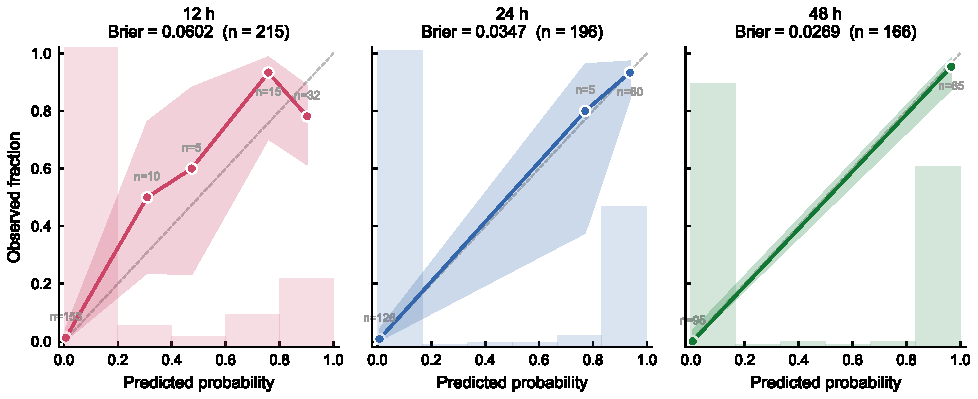
\includegraphics[width=\linewidth]{figures/main/Figure_3_reliability_diagrams.pdf}
\end{adjustwidth}
    \caption{Reliability diagrams for 12, 24, and 48~h horizons (pre-recalibration, nested OOF). Shaded bands represent Wilson confidence intervals. Histograms show predicted probability distributions. The dashed diagonal indicates perfect calibration.}\label{fig:reliability}
\end{figure}

Calibration was best at 24~h (slope~=~0.998; ECE~=~0.014), consistent with near-perfect diagonal alignment in the reliability diagram.
At 48~h, calibration was acceptable (slope~=~1.075, slightly underconfident; ECE~=~0.031).
The 12~h horizon proved the most challenging, with a slope of 0.805 indicating moderate overconfidence and an ECE of 0.057---consistent with the inherent difficulty of calibrating short-horizon predictions.
Horizon-wise trends in Brier score, ECE, and calibration slope are summarised in Figure~\ref{fig:calsummary}.
The maximum calibration error (MCE) increased with longer horizons (0.556 at 12~h to 0.777 at 48~h), reflecting sparse high-probability bins where individual deviations can be large even when average calibration is good.
The calibration intercept shifted from positive at 12~h (0.245, underestimation) to negative at 48~h ($-$0.272, overestimation), a pattern likely amplified by the monotone fusion constraint propagating probabilities forward.
Operationally, the 24~h horizon provides the most reliable absolute probability outputs; the 12~h outputs require caution for threshold-based triggers, with post-fusion recalibration assessed in Section~\ref{sec:recal_results}.

\begin{figure}[!ht]
\begin{adjustwidth}{-\extralength}{0cm}
    \centering
    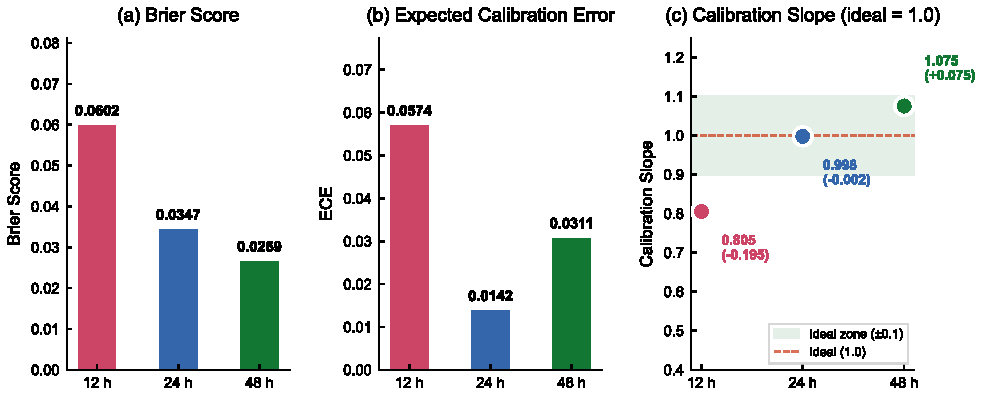
\includegraphics[width=\linewidth]{figures/main/Figure_4_calibration_summary.pdf}
\end{adjustwidth}
    \caption{Calibration summary: (a)~Brier score, (b)~expected calibration error (ECE), and (c)~calibration slope by horizon. The dashed line in~(c) indicates the ideal slope of 1.0.}\label{fig:calsummary}
\end{figure}

\subsection{Baseline Comparison}\label{sec:baseline_results}

Table~\ref{tab:baseline} and Figure~\ref{fig:baseline} present the baseline comparison.

\begin{table}[!ht]
\caption{Core model comparison (all models evaluated under the same nested OOF protocol, seed~=~42). IBS = mean Brier score across 12/24/48~h horizons. Uno-C = Uno's IPCW C-index. Models are grouped by role: physics-informed baseline, survival-centred lean variants, external comparators, and the full prototype.}\label{tab:baseline}
\begin{adjustwidth}{-0.5\extralength}{-0.5\extralength}
\centering
\footnotesize
\begin{tabular}{llcccccc}
\toprule
\textbf{Role} & \textbf{Model} & \textbf{C-index} & \textbf{Uno-C} & \textbf{IBS} & \textbf{Brier@12\,h} & \textbf{Brier@24\,h} & \textbf{Brier@48\,h} \\
\midrule
Baseline          & ETA-only (LR)            & 0.908 & 0.910 & 0.045 & 0.070 & 0.038 & 0.028 \\
\midrule
\multirow{3}{*}{\parbox{1.6cm}{Lean\\variants}} 
                  & AFT Only                 & 0.938 & 0.940 & 0.039 & 0.055 & 0.035 & 0.027 \\
                  & AFT + Cox                & 0.939 & 0.940 & 0.039 & 0.055 & 0.035 & 0.027 \\
                  & AFT + Cox + Simple       & 0.941 & 0.942 & 0.038 & 0.055 & 0.035 & 0.025 \\
\midrule
\multirow{2}{*}{\parbox{1.6cm}{External\\comparators}}
                  & Per-horizon XGBoost      & 0.942 & 0.943 & 0.040 & 0.056 & 0.037 & 0.026 \\
                  & Random Survival Forest   & 0.940 & 0.941 & 0.032 & 0.051 & 0.028 & 0.018 \\
\midrule
Prototype         & Full Model               & 0.940 & 0.941 & 0.041 & 0.060 & 0.035 & 0.027 \\
\bottomrule
\end{tabular}
\end{adjustwidth}
\end{table}

\begin{figure}[!ht]
\begin{adjustwidth}{-\extralength}{0cm}
    \centering
    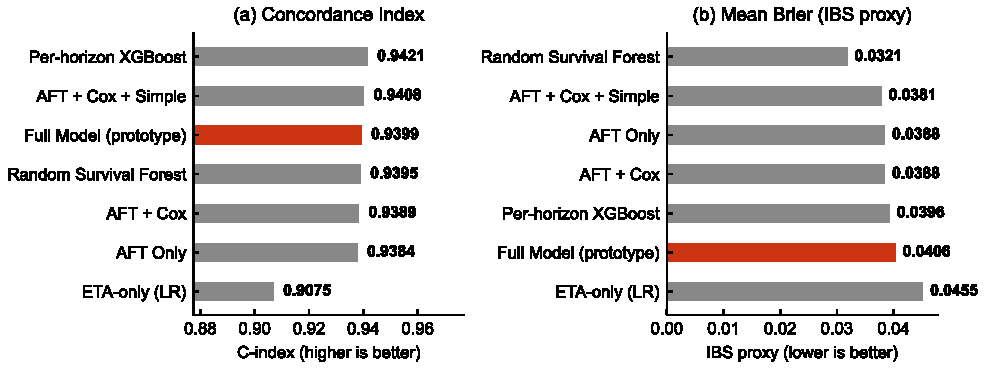
\includegraphics[width=\linewidth]{figures/main/Figure_5_baseline_comparison.pdf}
\end{adjustwidth}
    \caption{Baseline comparison: (a)~pairwise concordance index proxy and (b)~integrated Brier score proxy. Higher C-index and lower IBS are better.}\label{fig:baseline}
\end{figure}

The full prototype substantially outperformed the physics-informed ETA-only baseline ($\Delta$C-index = +0.032) but did not uniformly dominate the stronger alternatives.
At this sample size, the framework's value lies in its coherent censor-aware structure rather than aggregate metric superiority.
Table~\ref{tab:baseline} organises the models into three functional tiers.

Among the \emph{lean AFT-centred variants}, AFT~+~Cox achieved discrimination (C-index: 0.939) close to the full model.
AFT~+~Cox~+~Simple achieved lower IBS (0.038 vs.\ 0.041), suggesting that the simple distance branch anchors probability estimates.
As expected by design, AFT~Only and AFT~+~Cox yielded identical Brier scores and calibration metrics, differing only in C-index---the Cox branch enters only the ranking signal.

Among the \emph{external comparators}, per-horizon XGBoost achieved the highest C-index (0.942) with comparable IBS (0.040), demonstrating that a well-tuned single-model approach can match the full framework at this sample size.
The Random Survival Forest (C-index: 0.940, IBS: 0.032) achieved the lowest probability error of any model tested.

From the paired bootstrap analysis, the $\Delta$C-index between the full model and AFT-only was +0.002 [$-$0.002, +0.004] ($p = 0.170$), and $\Delta$IBS was $-$0.002 ($p = 0.805$), both non-significant.
The comparison with RSF is more nuanced: RSF is itself censor-aware with inherently monotone probabilities.
At this data scale, RSF's superior IBS and greater seed stability suggest that a single unified survival model absorbs the available signal more efficiently than the full stacked architecture, while the framework's modular design remains a research-oriented advantage requiring confirmation on larger datasets.

\subsection{Ablation Study}\label{sec:ablation_results}

Figure~\ref{fig:ablation} presents the ablation forest plot, and Table~\ref{tab:ablation} reports detailed results.

\begin{figure}[!ht]
\begin{adjustwidth}{-\extralength}{0cm}
    \centering
    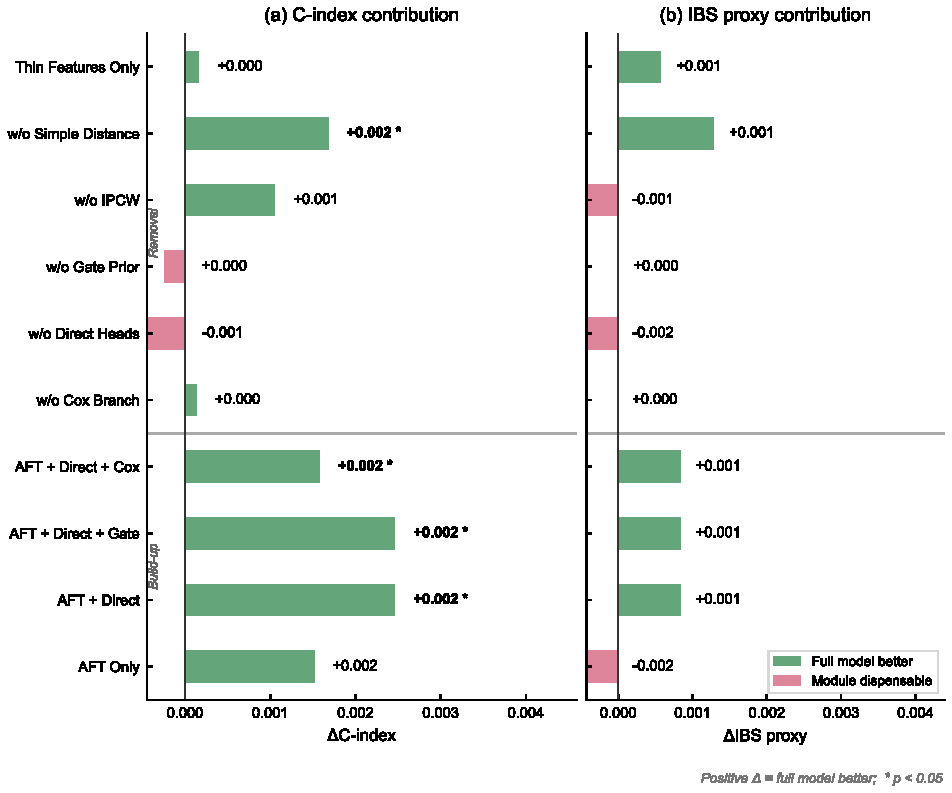
\includegraphics[width=\linewidth]{figures/main/Figure_6_ablation_contribution_summary.pdf}
\end{adjustwidth}
    \caption{Ablation forest plot showing the contribution of each configuration relative to the full model ($\Delta$C-index and $\Delta$IBS). Positive values indicate that the full model outperformed the ablated variant. Asterisks denote significance at $p < 0.05$ from paired bootstrap.}\label{fig:ablation}
\end{figure}

\begin{table}[!ht]
\caption{Ablation study: paired delta-metric bootstrap results (1000 resamples). $\Delta > 0$ indicates full model superiority. CI = 95\% bootstrap confidence interval. $p$ = one-sided. Significance: * $p < 0.05$.}\label{tab:ablation}
\small
\begin{tabular}{lcccc}
\toprule
\textbf{Configuration} & \textbf{$\Delta$C-index [95\% CI]} & \textbf{$p$} & \textbf{$\Delta$IBS [95\% CI]} & \textbf{$p$} \\
\midrule
AFT Only           & +0.002 [$-$0.002, +0.004] & 0.340 & $-$0.002 [$-$0.006, +0.003] & 0.390 \\
AFT + Direct       & +0.002 [+0.000, +0.005]* & 0.024 & +0.001 [$-$0.002, +0.004] & 0.588 \\
AFT + Direct + Cox & +0.002 [$-$0.000, +0.003] & 0.096 & +0.001 [$-$0.002, +0.004] & 0.588 \\
AFT + Direct + Gate & +0.002 [+0.000, +0.005]* & 0.024 & +0.001 [$-$0.002, +0.004] & 0.588 \\
w/o Gate Prior     & $-$0.000 [$-$0.001, +0.000] & 0.064 & +0.000 [$-$0.000, +0.000] & 0.524 \\
w/o Cox Branch     & +0.000 [$-$0.002, +0.002] & 0.892 & +0.000 [+0.000, +0.000] & $<$0.001 \\
w/o IPCW           & +0.001 [$-$0.000, +0.002] & 0.110 & $-$0.001 [$-$0.002, +0.001] & 0.400 \\
w/o Simple Dist.   & +0.002 [+0.000, +0.004]* & 0.050 & +0.001 [$-$0.001, +0.004] & 0.312 \\
w/o Direct Heads   & $-$0.001 [$-$0.003, +0.001] & 0.422 & $-$0.002 [$-$0.005, +0.001] & 0.126 \\
Thin Features      & +0.000 [$-$0.006, +0.006] & 0.964 & +0.001 [$-$0.005, +0.006] & 0.834 \\
\bottomrule
\end{tabular}
\end{table}

Among the modular configurations tested in the ablation study, the complete framework showed a numerically favourable discrimination profile, though external baselines such as per-horizon XGBoost and RSF achieved comparable or superior aggregate metrics (see Section~\ref{sec:baseline_results}).
The ablation results reveal heterogeneous module contributions.
Removing the \emph{Cox branch} yielded $\Delta$C-index = +0.000 ($p = 0.892$) and $\Delta$IBS exactly zero ($p < 0.001$), confirming by design that it affects only the ranking signal.
The \emph{simple distance branch} contributed to both discrimination and probability error ($\Delta$C-index = +0.002, $p = 0.050$; $\Delta$IBS = +0.001, $p = 0.312$).
The \emph{gate prior} and \emph{IPCW} modules showed limited independent gains; their effects may be absorbed by remaining components or emerge with more data.

The build-up analysis revealed that AFT~+~Direct exhibited a significant deficit relative to the full model ($\Delta$C-index = +0.002, $p = 0.024$), while AFT-only showed a comparable but non-significant gap ($\Delta = +0.002$, $p = 0.340$).
This pattern suggests that direct heads introduce estimation variance that the complementary modules (Cox, gate prior, IPCW, simple distance) compensate for in the full configuration---consistent with the observation that removing direct heads marginally improved IBS ($\Delta = -0.002$, $p = 0.126$).
Adding the Cox branch to AFT~+~Direct reduced the C-index gap ($p = 0.096$), consistent with its role as a discrimination enhancer.

\subsection{Bootstrap Confidence Intervals}\label{sec:bootstrap}

Bootstrap distributions for the primary metrics are shown in Figure~\ref{fig:bootstrap}.
The C-index distribution (median~=~0.940, 95\% CI: [0.927,~0.955]) was tightly concentrated, and the Uno's IPCW C-index (0.941, [0.924,~0.959]) confirmed consistent censoring-adjusted discrimination.
The IBS proxy (0.041, [0.025,~0.058]) and horizon-specific Brier distributions showed low probability error with moderate CI width reflecting the sample size.
All distributions are based on pre-recalibration predictions.

\begin{figure}[!ht]
\begin{adjustwidth}{-\extralength}{0cm}
    \centering
    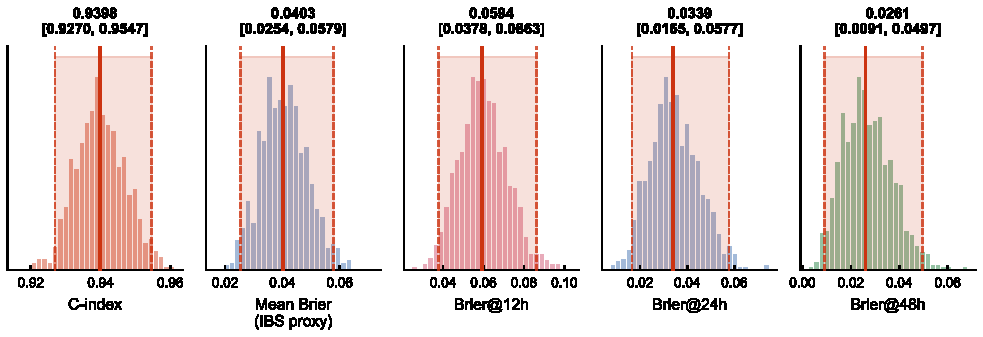
\includegraphics[width=\linewidth]{figures/main/Figure_7_bootstrap_confidence_intervals.pdf}
\end{adjustwidth}
    \caption{Bootstrap confidence interval distributions (1000 stratified resamples, pre-recalibration) for primary performance metrics. Solid red lines indicate medians; dashed red lines indicate the 2.5th and 97.5th percentiles defining 95\% CIs. Shaded bands span the CI region.}\label{fig:bootstrap}
\end{figure}

\subsection{Risk Stratification and Monotonicity}\label{sec:stratification}

After monotone-constrained fusion (Module~D), zero violations of $P(T \leq h_1) \leq P(T \leq h_2)$ remained across all 221 observations---by construction.
The more informative diagnostic is the \emph{pre-fusion} violation rate: zero violations occurred at the 12~h~$\to$~24~h transition, but 55/221 (24.9\%) at 24~h~$\to$~48~h, with a mean absolute adjustment of 0.002 (max: 0.115).
Without monotone enforcement, approximately one-quarter of observations would have received logically incoherent probability sequences at the 24--48~h transition, confirming that the enforcement module plays a substantive corrective role rather than serving as a formality.
Scatter plots are provided in Figure~S1.

Risk stratification based on 24~h predicted probability terciles produced highly separated observed event rates (Table~\ref{tab:stratification}; Figure~\ref{fig:distributions}).
The low-risk group ($n = 65$) experienced no events within 24~h (0.0\%; 95\% Wilson CI: 0.0--5.6\%), the medium-risk group ($n = 66$) had a 4.5\% event rate (CI: 1.6--12.5\%), and the high-risk group ($n = 65$) experienced events in 92.3\% of cases (CI: 83.2--96.7\%).
These tercile cutpoints were derived from the OOF predictions and should be regarded as data-dependent; their stability across repeated cross-validation splits has not been formally assessed.

\begin{table}[!ht]
\caption{Risk stratification by 24~h predicted probability terciles. Event rates and 95\% Wilson confidence intervals are computed on the censor-aware eligible subset ($n = 196$).}\label{tab:stratification}
\begin{tabular}{lccc}
\toprule
\textbf{Risk Tercile} & \textbf{$n$} & \textbf{Observed Event Rate (\%)} & \textbf{95\% Wilson CI} \\
\midrule
Low    & 65 & 0.0  & [0.0, 5.6] \\
Medium & 66 & 4.5  & [1.6, 12.5] \\
High   & 65 & 92.3 & [83.2, 96.7] \\
\bottomrule
\end{tabular}
\end{table}

\begin{figure}[!ht]
\begin{adjustwidth}{-\extralength}{0cm}
    \centering
    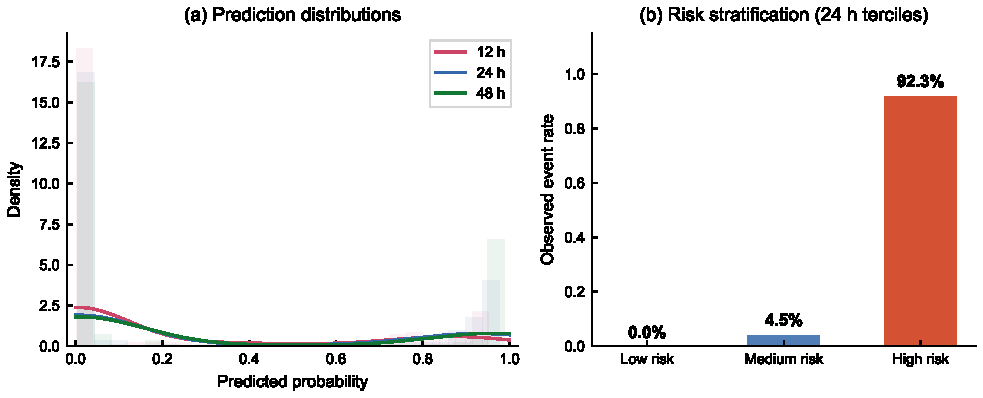
\includegraphics[width=\linewidth]{figures/main/Figure_8_prediction_distributions_and_risk_stratification.pdf}
\end{adjustwidth}
    \caption{(a)~Predicted probability distributions across the three horizons. The bimodal pattern reflects the clear separation between low- and high-threat cases under monotone-constrained fusion, consistent with the strong risk stratification observed in the data. (b)~Risk stratification by 24~h predicted probability terciles, with observed event rates of 0.0\% (low), 4.5\% (medium), and 92.3\% (high risk).}\label{fig:distributions}
\end{figure}

\subsection{Practical Lean Variants and Model Simplification}\label{sec:lean_results}

Table~\ref{tab:baseline} includes the lean AFT-centred variants alongside the external comparators and the full prototype.
Paired bootstrap comparisons yielded non-significant differences for both lean variants: AFT~+~Cox vs.\ Full Model ($\Delta$C-index = +0.001, $p = 0.260$; $\Delta$IBS = $-$0.002, $p = 0.805$) and AFT~+~Cox~+~Simple vs.\ Full Model ($\Delta$C-index = $-$0.001, $p = 0.762$; $\Delta$IBS = $-$0.002, $p = 0.869$), with the latter achieving numerically lower IBS (0.038 vs.\ 0.041).

These results confirm that the additional modules (direct heads, gate prior, IPCW) do not yield statistically significant gains given the available data.
The Cox branch's contribution was confined to discrimination (C-index 0.939 vs.\ 0.938 for AFT~Only, identical probability metrics).
The simple distance branch improved probability error without affecting discrimination (IBS = 0.038 vs.\ 0.039 for AFT~+~Cox).

\subsection{Multi-Seed Stability Analysis}\label{sec:stability}

Table~\ref{tab:stability} summarises the multi-seed stability results across five random seeds.

\begin{table}[!ht]
\caption{Multi-seed stability analysis (five seeds: 42, 123, 314, 2024, 7777). Mean and standard deviation of C-index and IBS proxy across seeds.}\label{tab:stability}
\begin{tabular}{lcc}
\toprule
\textbf{Model} & \textbf{C-index (mean $\pm$ SD)} & \textbf{IBS (mean $\pm$ SD)} \\
\midrule
Random Survival Forest & 0.941 $\pm$ 0.001 & 0.032 $\pm$ 0.000 \\
Per-horizon XGBoost    & 0.940 $\pm$ 0.001 & 0.039 $\pm$ 0.001 \\
AFT + Cox + Simple     & 0.939 $\pm$ 0.003 & 0.040 $\pm$ 0.001 \\
Full Model (prototype) & 0.938 $\pm$ 0.003 & 0.041 $\pm$ 0.002 \\
AFT + Cox              & 0.938 $\pm$ 0.003 & 0.040 $\pm$ 0.002 \\
\bottomrule
\end{tabular}
\end{table}

RSF exhibited the smallest variability (C-index SD = 0.001; IBS SD $<$ 0.001), followed by per-horizon XGBoost (C-index SD = 0.001; IBS SD = 0.001).
The full model and lean AFT variants showed greater seed-to-seed variability (C-index SD = 0.003; IBS SD = 0.001--0.002), consistent with higher estimation variance from multi-module stacking on a small dataset.
RSF ranked first or second in four of five seeds; the full model fluctuated between first and fourth.
These findings confirm that performance differences among survival-based models fall within the noise margin at $n = 221$.

\subsection{Sensitivity Analysis: Joint Post-Fusion Recalibration}\label{sec:recal_results}

The joint post-fusion recalibration sensitivity analysis identified an optimal temperature of $T = 1.50$ for the 12~h horizon.
Table~\ref{tab:recalibration} and Figure~\ref{fig:recalibration} compare pre- and post-recalibration metrics.

\begin{table}[!ht]
\caption{Pre- vs.\ post-recalibration comparison. Joint = joint post-fusion temperature scaling; 12h-only = legacy 12~h-only temperature scaling.}\label{tab:recalibration}
\begin{tabular}{lcccccccc}
\toprule
 & \multicolumn{3}{c}{\textbf{Brier Score}} & \multicolumn{3}{c}{\textbf{ECE}} & \multicolumn{2}{c}{\textbf{Cal.\ Slope}} \\
\cmidrule(lr){2-4} \cmidrule(lr){5-7} \cmidrule(lr){8-9}
\textbf{Horizon} & Pre & Joint & 12h-only & Pre & Joint & 12h-only & Pre & Joint \\
\midrule
12~h & 0.060 & 0.058 & 0.059 & 0.057 & 0.048 & 0.048 & 0.805 & 0.964 \\
24~h & 0.035 & 0.035 & 0.035 & 0.014 & 0.010 & 0.019 & 0.998 & 1.014 \\
48~h & 0.027 & 0.027 & 0.027 & 0.031 & 0.031 & 0.037 & 1.075 & 1.052 \\
\midrule
IBS proxy & 0.041 & 0.040 & 0.040 & --- & --- & --- & --- & --- \\
\bottomrule
\end{tabular}
\end{table}

\begin{figure}[!ht]
\begin{adjustwidth}{-\extralength}{0cm}
    \centering
    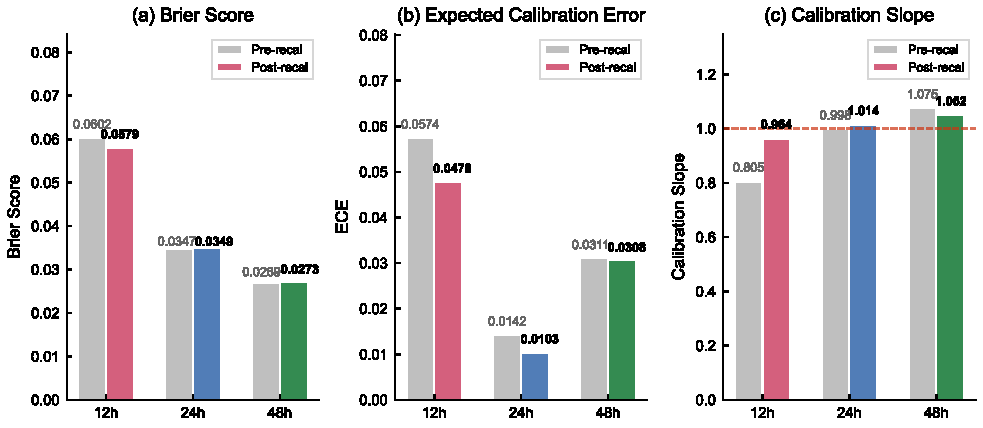
\includegraphics[width=\linewidth]{figures/main/Figure_9_pre_vs_post_recalibration.pdf}
\end{adjustwidth}
    \caption{Pre- vs.\ post-recalibration comparison: (a)~Brier score, (b)~ECE, and (c)~calibration slope. Grey bars represent pre-recalibration values; coloured bars represent post-recalibration values.}\label{fig:recalibration}
\end{figure}

Joint post-fusion recalibration reduced the 12~h Brier score from 0.060 to 0.058 and ECE from 0.057 to 0.048, moving the calibration slope from 0.805 to 0.964---close to the ideal.
The overall IBS proxy decreased from 0.041 to 0.040.
Crucially, this approach preserved calibration at 24~h and 48~h (24~h ECE improved from 0.014 to 0.010; 48~h ECE unchanged at 0.031).
The legacy 12~h-only variant over-corrected (slope = 1.209) and slightly degraded 24~h and 48~h ECE, confirming that joint recalibration is preferable for multi-horizon pipelines.
The improvement is modest, and recalibration is retained as a sensitivity analysis rather than replacing the primary model.

\subsection{Robustness Checks for Validation Bias and Censoring Assumptions}\label{sec:robustness_results}

Because verified wildfire-incident identifiers were unavailable, auxiliary robustness checks were conducted with a lean AFT model.
Under proxy incident-grouped cross-validation, the mean C-index decreased modestly from 0.9318 $\pm$ 0.0119 (standard stratified CV) to 0.9283 $\pm$ 0.0323 (grouped CV), while the mean Brier score increased from 0.1352 $\pm$ 0.0341 to 0.1541 $\pm$ 0.0761 (Supplementary Table~S8).
The limited C-index drop suggests that major leakage-driven optimism is unlikely, but the grouped split produced worse probability error and substantially wider fold-to-fold variability.
A leave-one-month-out temporal blocked analysis yielded an $N$-weighted mean C-index of 0.935 across six months with $\geq$10 observations.
The three largest holdout months (Jun--Aug; $n = 33$--70) fell within $C = 0.923$--0.943, while smaller months were more variable, including a likely artefactual March estimate of $C = 1.000$.

Regarding the censoring assumption, worst-case/best-case event-rate bounds showed sensitivity ranges of 0.027 at 12~h, 0.113 at 24~h, and 0.249 at 48~h, with the 48~h base event rate spanning 0.299--0.548 under extreme scenarios (Supplementary Table~S9).
Short-horizon estimates are thus relatively stable, whereas 48~h outputs are materially more assumption-sensitive.
Figure~\ref{fig:robustness} summarises these diagnostics; standalone versions are in Supplementary Figures~S2 and~S4.

\begin{figure}[!ht]
\begin{adjustwidth}{-\extralength}{0cm}
    \centering
    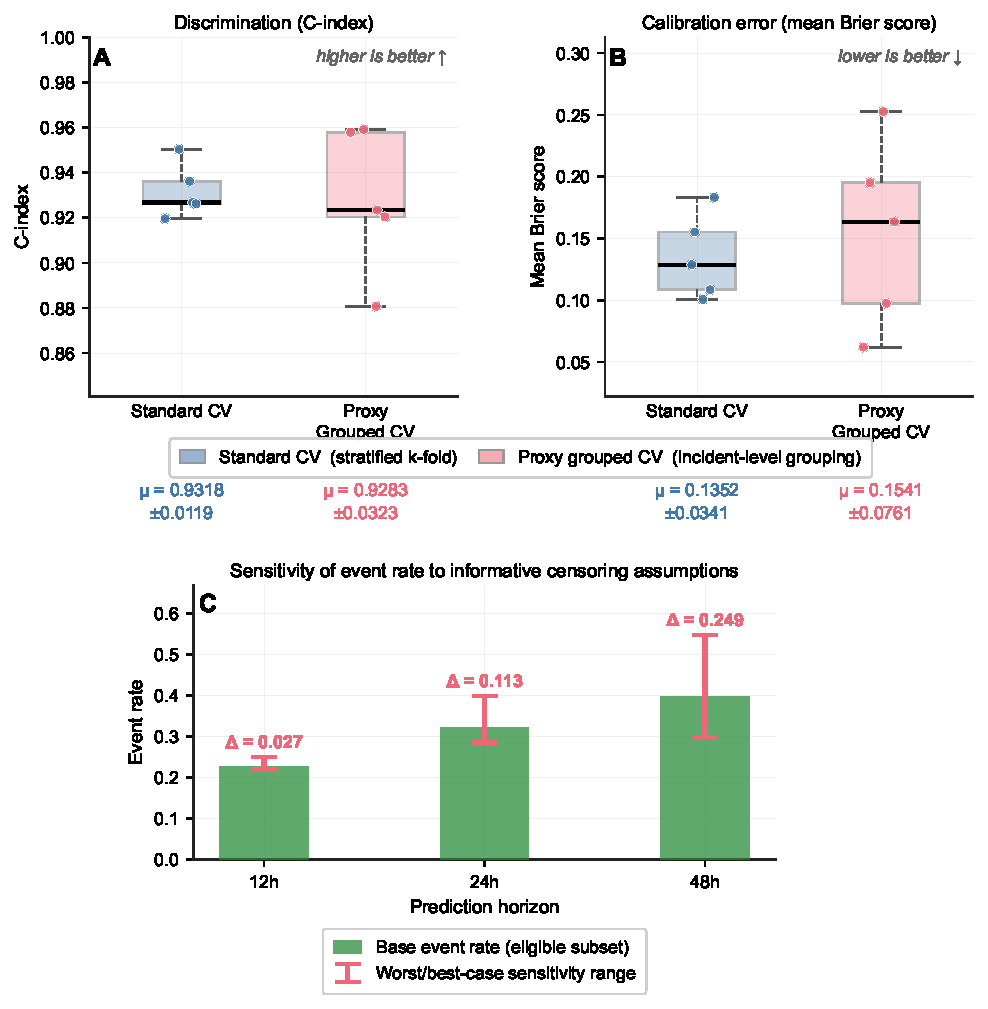
\includegraphics[width=\linewidth]{figures/main/Figure_10_robustness_diagnostics.pdf}
\end{adjustwidth}
    \caption{Main-text robustness diagnostics derived from auxiliary lean-model checks. (a)~Discrimination (C-index) under standard stratified versus proxy incident-grouped cross-validation. (b)~Mean Brier score under the same validation splits, showing worse probability error and greater variability under grouped splitting. (c)~Sensitivity of horizon-specific event rates to informative-censoring assumptions, shown as worst/best-case ranges around the base event rate; the widest range occurs at 48~h. Standalone full-page versions are provided as Supplementary Figures~S2 and~S4.}\label{fig:robustness}
\end{figure}

\subsection{Decision Curve Analysis and Decision Utility}\label{sec:dca_results}

To evaluate the framework's potential value for threshold-based decision-making, decision curve analysis (DCA)~\cite{Vickers2006} was conducted at all three primary horizons.
Table~\ref{tab:dca_utility} presents decision utility metrics at selected thresholds, and the net benefit across the full threshold range is reported in Supplementary Table~S5.

\begin{table}[!ht]
\caption{Decision utility at selected probability thresholds (pre-recalibration, nested OOF). Sens.\ = sensitivity; Spec.\ = specificity; PPV = positive predictive value; NPV = negative predictive value; NB = net benefit.}\label{tab:dca_utility}
\small
\begin{tabular}{lccccccc}
\toprule
\textbf{Horizon} & \textbf{Threshold} & \textbf{Sens.} & \textbf{Spec.} & \textbf{PPV} & \textbf{NPV} & \textbf{F1} & \textbf{NB} \\
\midrule
12~h & 0.1 & 0.959 & 0.886 & 0.712 & 0.987 & 0.817 & 0.209 \\
12~h & 0.3 & 0.939 & 0.928 & 0.793 & 0.981 & 0.860 & 0.190 \\
12~h & 0.5 & 0.796 & 0.946 & 0.813 & 0.940 & 0.804 & 0.140 \\
\midrule
24~h & 0.1 & 0.984 & 0.932 & 0.873 & 0.992 & 0.925 & 0.311 \\
24~h & 0.3 & 0.984 & 0.940 & 0.886 & 0.992 & 0.932 & 0.299 \\
24~h & 0.5 & 0.968 & 0.955 & 0.910 & 0.984 & 0.938 & 0.281 \\
\midrule
48~h & 0.1 & 1.000 & 0.950 & 0.930 & 1.000 & 0.964 & 0.394 \\
48~h & 0.3 & 0.985 & 0.950 & 0.929 & 0.990 & 0.956 & 0.379 \\
48~h & 0.5 & 0.970 & 0.960 & 0.941 & 0.980 & 0.955 & 0.361 \\
\bottomrule
\end{tabular}
\end{table}

The model produced positive net benefit exceeding both ``treat-all'' and ``treat-none'' strategies across a wide threshold range at all three horizons.
At the best-calibrated 24~h horizon, a threshold of 0.3 yielded sensitivity of 0.984, specificity of 0.940, and net benefit of 0.299.
The 48~h horizon showed the highest net benefit (0.394 at threshold 0.1), reflecting higher base rates.
Even the 12~h horizon, despite weaker calibration, maintained positive net benefit up to threshold $\approx$ 0.8, supporting its use for relative triage.

\subsection{Feature Importance}\label{sec:feature_importance}

Gain-based feature importance from the AFT backbone (Table~\ref{tab:feature_importance}) confirmed that distance-related features dominated: log-distance (gain = 20.0), minimum perimeter distance (10.5), and low temporal resolution (8.9) occupied the top three positions.
The dominance of distance features is physically intuitive---proximity to the fire front is the strongest predictor of zone-level threat.
The prominence of temporal resolution and perimeter count suggests that data quality indicators also carry predictive information, likely proxying for fire complexity or monitoring intensity.

\begin{table}[!ht]
\caption{Top 10 features by AFT gain-based importance.}\label{tab:feature_importance}
\begin{tabular}{lc}
\toprule
\textbf{Feature} & \textbf{Gain} \\
\midrule
Log-distance              & 20.00 \\
Min distance to perimeter & 10.48 \\
Low temporal resolution   &  8.91 \\
Number of perimeters      &  3.63 \\
Inverse distance          &  3.42 \\
Time span (first--last)   &  2.01 \\
Short-range urgency       &  0.99 \\
Cross-track component     &  0.89 \\
Month (sine)              &  0.73 \\
Start month               &  0.71 \\
\bottomrule
\end{tabular}
\end{table}

\section{Discussion}\label{sec:discussion}

This study presented a survival--probability fusion framework for censor-aware multi-horizon wildfire threat forecasting, evaluated on a dataset whose modest size (221 observations, 69 events, EPV~$\approx$~2.0) constrains how firmly the full architecture's merits can be established.
The framework achieved strong discrimination (Uno-C = 0.941), low probability error (Brier 0.027--0.060), enforced monotonicity, and sharp risk stratification (24~h tercile event rates: 0.0\%, 4.5\%, 92.3\%), with calibration quality best at 24~h (slope = 0.998) and weakest at 12~h (slope = 0.805).
However, the full model did not outperform all alternatives: RSF achieved lower probability error, per-horizon XGBoost achieved marginally higher discrimination, and lean AFT variants remained competitive.
The primary contribution is therefore methodological: the framework provides an architectural template for combining censor-aware survival modelling with calibrated multi-horizon output, and the evaluation transparently characterises when simpler alternatives are preferable.

\paragraph{Three-tier model roles.}
The models fall into three functional tiers.
The \emph{full model} is a methodological prototype demonstrating the integration of censor-aware survival modelling, horizon-targeted heads, monotone enforcement, and modular ablation.
The \emph{lean AFT variants} (AFT~+~Cox, AFT~+~Cox~+~Simple) are interim practical alternatives preserving censor-awareness and monotone coherence at substantially reduced complexity.
The \emph{Random Survival Forest} is the strongest practical comparator at this data scale, combining the lowest IBS (0.032) with the highest seed-to-seed stability.
RSF is itself censor-aware with naturally monotone probabilities; the framework's distinction lies in its modular fusion architecture and horizon-targeted calibration pipeline.

\paragraph{Framework design and ablation insights.}
Existing wildfire threat models have focused on spatial susceptibility mapping at a single horizon~\cite{Jaafari2019,Gigovic2019,Chen2024wui,Kaur2022} or physics-based fire-spread simulation~\cite{Finney2001,Cruz2003,Shu2020,Pais2021,Zheng2021}, neither producing calibrated multi-horizon probabilities under censoring.
Evacuation decision support has been studied through vulnerability assessments and trigger-point analyses~\cite{Dolan2022,Paveglio2019,Alcasena2019}, and time-to-event perspectives appear in the broader wildfire risk literature~\cite{Xi2019,Taylor2013}, but zone-level threat prediction with calibrated multi-horizon output under censoring has not been previously addressed.

A key empirical finding is that explicit monotone enforcement is necessary in stacked multi-horizon setups: approximately 25\% of observations at the 24--48~h transition exhibited incoherent probability sequences before fusion.
The ablation results further show that direct heads require complementary modules to function effectively: AFT~+~Direct showed a significant C-index deficit ($p = 0.024$) while AFT-only showed a non-significant deficit ($p = 0.340$), indicating that direct heads alone introduce variance that the remaining modules compensate for.
This synergistic pattern supports a modular design where individual contributions are not strictly additive.

\paragraph{Module prioritisation under low EPV.}
Combining evidence from the ablation, lean-variant, and stability analyses, the most defensible reduced architecture at EPV~$\approx$~2.0 centres on the AFT backbone with optional Cox (for discrimination) and simple distance (for probability anchoring).
The gate prior, IPCW, and direct heads showed limited independent gains at this scale; their incremental value requires confirmation on larger datasets.

\paragraph{Calibration and horizon-level deployment readiness.}
The calibration metrics in Table~\ref{tab:calibration} refer to the final fused probabilities.
The 12~h horizon is inherently the hardest to calibrate; its slope of 0.805 reflects moderate overconfidence, meaning threshold-based triggers at 12~h require recalibration.
A structural factor contributes: beta calibration targets each base head independently, but stacking and monotone fusion subsequently reshape the distribution.
Joint post-fusion temperature scaling corrected the 12~h slope to 0.964 without degrading other horizons (Table~\ref{tab:recalibration}), confirming that multi-horizon frameworks benefit from joint recalibration strategies~\cite{NiculescuMizil2005}.
The 24~h slope of 0.998 makes it the most promising horizon for threshold-based decisions.
The 48~h slope of 1.075 indicates slight conservatism, compounded by greater censoring sensitivity (sensitivity range = 0.249).
Improving 12~h calibration without degrading longer horizons could be further pursued through bidirectional monotone adjustment or soft monotone penalties during stacking optimisation.

\paragraph{Practical model selection.}
At EPV~$\approx$~2.0, the full framework's architectural advantages did not translate into significant aggregate gains over leaner alternatives ($\Delta$C-index vs.\ AFT-only: $+0.002$, $p = 0.340$; $\Delta$IBS: $-0.002$, $p = 0.390$).
The most defensible interim choices are lean AFT variants when modularity is desired, or RSF when predictive robustness is prioritised.

\paragraph{Validation and censoring robustness.}
The proxy incident-grouped analysis showed a modest mean C-index decrease relative to standard stratified CV, suggesting that major leakage-driven inflation is unlikely, though the grouped split worsened mean Brier score and widened fold-to-fold variability.
Temporal blocking produced similar discrimination in the three largest fire-season months (Jun--Aug), but smaller holdouts remained unstable.
Informative-censoring sensitivity increased monotonically with horizon length: the 48~h event-rate estimate spanned 29.9\%--54.8\% under extreme assumptions, reinforcing 24~h as the most defensible operational horizon.

\paragraph{Practical implications.}
The risk stratification capability may be the most actionable contribution: a wildfire--zone pair at 3200~m with closing speed 400~m/h and growth rate 50~ha/h would yield fused probabilities of approximately $P(T \leq 12) = 0.72$, $P(T \leq 24) = 0.91$, $P(T \leq 48) = 0.95$, placing it in the high-risk tercile.
The 24~h tercile separation (0.0\% vs.\ 92.3\%) supports a triage protocol: high-risk zones receive immediate pre-evacuation preparation, medium-risk zones go on standby, and low-risk zones remain at routine surveillance.
This tercile-based approach is more robust than raw probability thresholds because it relies on ranking ability (C-index = 0.941) rather than absolute calibration.
Decision curve analysis confirmed positive net benefit across a wide threshold range, with sensitivity~$>$~0.98 and specificity~$>$~0.93 at operationally relevant thresholds (e.g., 0.3 at 24~h).
The framework is positioned as a decision-support tool; deployment would require integration with near-real-time fire-behaviour feeds~\cite{Radeloff2023} and evaluation against agency-specific thresholds.

\paragraph{Strengths and limitations.}
Strengths include the censor-aware problem formulation, nested cross-validation with inner cross-fitting, multi-horizon monotonicity enforcement, transparent metric proxy definitions, comprehensive ablation and baseline analyses, lean-variant evaluation, and five-seed stability analysis.
The candid acknowledgement that simpler alternatives matched or exceeded the full framework is itself informative for practitioners.
Future evaluations should include deep survival models (e.g., DeepSurv~\cite{Katzman2018}) and discrete-time hazard models for more demanding comparisons.

Several limitations warrant emphasis.
First, the sample size ($n = 221$, 69 events, EPV~$\approx$~2.0) is the most consequential constraint: it is insufficient to reliably support the full modelling complexity, and is the most parsimonious explanation for why the full model did not outperform simpler competitors~\cite{Riley2020}.
The low EPV also limits the stability of three-parameter beta calibration (effective inner-fold samples as low as $\sim$35), the precision of bootstrap CIs, and the statistical power of ablation tests.
Second, the outer CV folds were not grouped by verified wildfire incident identifier; proxy grouped-CV analysis suggested modest average optimism ($\Delta$C-index = $-$0.004), but formal incident-level validation remains necessary.
Third, no external spatiotemporal validation was conducted.
Fourth, fire containment may violate the independent censoring assumption; worst/best-case event-rate bounds widened from 0.027 at 12~h to 0.249 at 48~h, motivating censoring-robust methods or competing-risk formulations in future work.
Fifth, the 72~h horizon was degenerate.
Sixth, both concordance indices and the IBS proxy are approximations adopted for tractability~\cite{Harrell1996,Uno2011,Graf1999}.
Seventh, post-hoc temperature scaling is a sensitivity analysis introducing calibration trade-offs across horizons.
Finally, direct deployment would require incident-level and external validation, real-time data integration, and regulatory review.

\section{Conclusions}\label{sec:conclusions}

A survival--probability fusion framework was developed and internally validated for multi-horizon wildfire threat forecasting under right censoring, producing coherent, monotonic probability estimates at 12, 24, and 48~h with strong discrimination (Uno-C = 0.941), low probability error (Brier 0.027--0.060), and sharp risk stratification (24~h tercile event rates: 0.0\%, 4.5\%, 92.3\%).
The 24~h horizon emerged as the most reliable operational target (calibration slope = 0.998), while the 48~h horizon requires more cautious interpretation due to censoring sensitivity.

The primary contribution is methodological.
The framework establishes a structured template for censor-aware multi-horizon probability estimation with explicit monotone enforcement---an enforcement confirmed to correct incoherent sequences in approximately 25\% of observations.
At the present data scale (EPV~$\approx$~2.0), however, the full architecture did not outperform all alternatives: RSF achieved lower probability error and greater stability, and lean AFT variants matched the prototype's discrimination.
A simpler AFT-centred pipeline with monotone fusion---or an RSF---is therefore the more appropriate interim choice; the full architecture constitutes a research prototype whose incremental benefits await confirmation on larger datasets.

Future work should prioritise incident-level grouped validation with verified identifiers, external spatiotemporal validation across diverse fire regimes, joint post-fusion calibration under the monotone constraint, and comparison with discrete-time hazard and deep survival models~\cite{Katzman2018}.
Prospective evaluation in operational early warning settings, integrated with real-time fire-spread data, is the necessary next step toward deployment.

%=================================================================
% Back Matter
%=================================================================
\vspace{6pt}

\supplementary{The following supporting information is available in the public repository at \url{https://github.com/eee-afkk/wids2026-wildfire-survival}: Table~S0: Complete feature dictionary (name, type, transformation, source). Table~S1: 72~h horizon performance results. Table~S2: Full hyperparameter configurations for all models, including stacking regularisation sensitivity analysis ($\lambda \in \{0.1, 0.5, 1.0, 2.0, 5.0\}$). Table~S3: Two-sided $p$-values for all ablation paired bootstrap comparisons. Table~S4: Fold-level performance metrics (C-index and Brier scores per outer fold). Table~S5: Decision curve analysis net benefit across the full threshold range at 12, 24, and 48~h. Table~S6: Complete feature importance ranking (all features). Table~S7: Practical lean variant comparison with thin-feature configurations. Table~S8: Proxy incident-grouped cross-validation comparison (standard stratified CV vs.\ feature-space clustering GroupKFold; lean AFT model). Table~S9: Informative censoring sensitivity analysis---worst-case/best-case event-rate bounds and Aalen--Johansen competing-risk cumulative incidence by horizon. Table~S10: Leave-one-month-out temporal blocked cross-validation results (lean AFT model). Table~S11: TRIPOD-style data quality summary (missing rates, variable distributions). Figure~S1: Monotonicity verification scatter plots. Figure~S2: Proxy incident-grouped CV comparison---boxplots of C-index and mean Brier score under standard stratified vs.\ grouped cross-validation (43 feature-space proxy groups). Figure~S3: Leave-one-month-out temporal blocked CV---per-month C-index and mean Brier score (months with $n < 10$ excluded); the figure reports unweighted monthly means ($\bar{C} = 0.937$), whereas the main text reports the $N$-weighted mean ($C = 0.935$) to account for differing per-month sample sizes. Figure~S4: Informative censoring sensitivity---worst/best-case event-rate bounds and Kaplan--Meier vs.\ Aalen--Johansen cumulative incidence by horizon. Figure~S5: Kaplan--Meier survival function and event-time vs.\ censoring-time distributions. Figure~S6: Eligible sample size and event rate per prediction horizon. Figure~S7: NIFC WFIGS geographic context---western US wildfire incidents used for supplementary proxy incident grouping (note: the 2026 bar in the annual counts panel may represent a partial year in the downloaded open-data snapshot and should not be interpreted as an anomalous decline). The repository also contains non-numbered workflow support files (e.g., validation\_strategy\_summary.csv) for provenance and navigation; these are not part of the formal supplementary record.}

\authorcontributions{Conceptualization, Z.R.; Methodology, Z.R.; Software, Z.R.; Validation, Z.R.; Formal Analysis, Z.R.; Investigation, Z.R.; Data Curation, Z.R.; Writing---Original Draft Preparation, Z.R.; Writing---Review \& Editing, Z.R.; Visualization, Z.R. The author has read and agreed to the published version of the manuscript.}

\funding{This research received no external funding.}

\institutionalreview{Not applicable.}

\informedconsent{Not applicable.}

\dataavailability{Restrictions apply to the availability of the WiDS Datathon 2026 data used in this study. The data were obtained from the WiDS 2026 Datathon competition platform (\url{https://www.wids.io}) and are available from the provider subject to its terms of access. The analysis code and curated supplementary data files are openly available at \url{https://github.com/eee-afkk/wids2026-wildfire-survival} (DOI to be assigned upon acceptance). Random seeds and environment specifications are documented in the repository README to support reproducibility.}

\conflictsofinterest{The author declares no conflict of interest.}

\abbreviations{The following abbreviations are used in this manuscript:
AFT = Accelerated failure time;
CDF = Cumulative distribution function;
CI = Confidence interval;
DCA = Decision curve analysis;
ECE = Expected calibration error;
ETA = Estimated time of arrival;
GBC = Gradient boosting classifier;
HGB = Histogram gradient boosting classifier;
IBS = Integrated Brier score;
IPCW = Inverse probability of censoring weighting;
LR = Logistic regression;
MCE = Maximum calibration error;
NB = Net benefit;
NPV = Negative predictive value;
OOF = Out-of-fold;
PPV = Positive predictive value;
RSF = Random Survival Forest.
}

%=================================================================
% References — inline thebibliography (MDPI standard, most stable)
%=================================================================
\begin{adjustwidth}{-\extralength}{0cm}
\reftitle{References}

\begin{thebibliography}{99}

\bibitem{Finney2001}
Finney, M.A.
Design of regular landscape fuel treatment patterns for modifying fire growth and behavior.
\textit{For.\ Sci.} \textbf{2001}, \textit{47}, 219--228.

\bibitem{Xi2019}
Xi, D.D.; Taylor, S.W.; Woolford, D.G.; Dean, C.B.
Statistical models of key components of wildfire risk.
\textit{Annu.\ Rev.\ Stat.\ Appl.} \textbf{2019}, \textit{6}, 197--222.

\bibitem{Stephens2018}
Stephens, S.L.; Collins, B.M.; Fettig, C.J.; Finney, M.; Hoffman, C.; Knapp, E.E.; North, M.P.; Safford, H.; Wayman, R.B.
Operational approaches to managing forests of the future in the western United States through complementary fire and forest management strategies.
\textit{For.\ Ecol.\ Manag.} \textbf{2018}, \textit{432}, 987--998.

\bibitem{Jain2022}
Jain, P.; Castellanos-Acuna, D.; Coogan, S.C.P.; Abatzoglou, J.T.; Flannigan, M.D.
Observed increases in extreme fire weather driven by atmospheric humidity and temperature.
\textit{Nat.\ Clim.\ Change} \textbf{2022}, \textit{12}, 63--70.

\bibitem{Cunningham2024}
Cunningham, C.X.; Williamson, G.J.; Bowman, D.M.J.S.
Increasing frequency and intensity of the most extreme wildfires on Earth.
\textit{Nat.\ Ecol.\ Evol.} \textbf{2024}, \textit{8}, 1420--1425.

\bibitem{Turco2023}
Turco, M.; Jerez, S.; Augusto, S.; Tarín-Carrasco, P.; Ratola, N.; Jim\'enez-Guerrero, P.; Trigo, R.M.
Anthropogenic climate change impacts exacerbate summer forest fires in California.
\textit{Proc.\ Natl.\ Acad.\ Sci.\ USA} \textbf{2023}, \textit{120}, e2213815120.

\bibitem{Luo2024}
Luo, K.; Wang, X.; de~Jong, M.; Flannigan, M.
Drought triggers and sustains overnight fires in North America.
\textit{Nature} \textbf{2024}, \textit{627}, 321--327.

\bibitem{Jones2022}
Jones, M.W.; Abatzoglou, J.T.; Veraverbeke, S.; Andela, N.; Lasslop, G.; Forkel, M.; Smith, A.J.P.; Burton, C.; Betts, R.A.; van~der~Werf, G.R.; Sitch, S.; Canadell, J.G.; Sant\'\i n, C.; Kolden, C.; Doerr, S.H.; Le~Qu\'er\'e, C.
Global and regional trends and drivers of fire under climate change.
\textit{Rev.\ Geophys.} \textbf{2022}, \textit{60}, e2020RG000726.

\bibitem{Kolden2024}
Kolden, C.A.; Abatzoglou, J.T.; Jones, M.W.; Jain, P.
Wildfires in 2023.
\textit{Nat.\ Rev.\ Earth Environ.} \textbf{2024}, \textit{5}, 238--240.

\bibitem{Higuera2021}
Higuera, P.E.; Abatzoglou, J.T.
Record-setting climate enabled the extraordinary 2020 fire season in the western United States.
\textit{Glob.\ Change Biol.} \textbf{2021}, \textit{27}, 1--2.

\bibitem{Radeloff2023}
Radeloff, V.C.; Helmers, D.P.; Kramer, H.A.; Mockrin, M.H.; Alexandre, P.M.; Bar-Massada, A.; Butsic, V.; Hawbaker, T.J.; Martinuzzi, S.; Syphard, A.D.; Stewart, S.I.
Rising wildfire risk to houses in the United States, especially in grasslands and shrublands.
\textit{Science} \textbf{2023}, \textit{382}, 702--707.

\bibitem{Tonini2020}
Tonini, M.; D'Andrea, M.; Biondi, G.; Degli Esposti, S.; Ferrari, A.; Pedrazzoli, F.
A machine learning-based approach for wildfire susceptibility mapping: The case study of the Liguria region in Italy.
\textit{Geosciences} \textbf{2020}, \textit{10}, 105.

\bibitem{Cruz2003}
Cruz, M.G.; Alexander, M.E.; Wakimoto, R.H.
Assessing canopy fuel stratum characteristics in crown fire prone fuel types of western North America.
\textit{Int.\ J.\ Wildland Fire} \textbf{2003}, \textit{12}, 39--50.

\bibitem{Jaafari2019}
Jaafari, A.; Zenner, E.K.; Panahi, M.; Shahabi, H.
Hybrid artificial intelligence models based on a neuro-fuzzy network and adaboost algorithm for spatial prediction of wildfire probability.
\textit{J.\ Environ.\ Manag.} \textbf{2019}, \textit{233}, 32--44.

\bibitem{Gigovic2019}
Gigovi\'{c}, L.; Pourghasemi, H.R.; Drobnjak, S.; Bai, S.
Testing a new ensemble model based on SVM and random forest in forest fire susceptibility assessment and its mapping in Serbia's Tara National Park.
\textit{Forests} \textbf{2019}, \textit{10}, 408.

\bibitem{Chen2024wui}
Chen, B.; Jin, Y.; Scaduto, E.; Bhatt, U.; Goulden, M.; Veloz, S.; Moritz, M.
Wildfire risk for global wildland--urban interface areas.
\textit{Nat.\ Sustain.} \textbf{2024}, \textit{7}, 474--484.

\bibitem{Wiegrebe2024}
Wiegrebe, S.; Kopper, P.; Bischl, B.; Bender, A.
Deep learning for survival analysis: A review.
\textit{Artif.\ Intell.\ Rev.} \textbf{2024}, \textit{57}, 65.

\bibitem{Taylor2013}
Taylor, S.W.; Woolford, D.G.; Dean, C.B.; Martell, D.L.
Wildfire prediction to inform fire management: Statistical science challenges.
\textit{Stat.\ Sci.} \textbf{2013}, \textit{28}, 586--615.

\bibitem{VanCalster2019}
Van Calster, B.; McLernon, D.J.; van Smeden, M.; et~al.
Calibration: the Achilles heel of predictive analytics.
\textit{BMC Med.} \textbf{2019}, \textit{17}, 230.

\bibitem{Steyerberg2019}
Steyerberg, E.W.
\textit{Clinical Prediction Models: A Practical Approach to Development, Validation, and Updating}, 2nd~ed.;
Springer: Cham, Switzerland, 2019.

\bibitem{Collins2024}
Collins, G.S.; Moons, K.G.M.; Dhiman, P.; Riley, R.D.; et~al.
TRIPOD+AI statement: updated guidance for reporting clinical prediction models that use regression or machine learning methods.
\textit{BMJ} \textbf{2024}, \textit{385}, e078378.

\bibitem{Riley2020}
Riley, R.D.; Ensor, J.; Snell, K.I.E.; Harrell, F.E.; Martin, G.P.; Reitsma, J.B.; Moons, K.G.M.; Collins, G.; van Smeden, M.
Calculating the sample size required for developing a clinical prediction model.
\textit{BMJ} \textbf{2020}, \textit{368}, m441.

\bibitem{Dolan2022}
Dolan, R.W.; Hammersley, L.A.; McKinley, C.M.
Evacuation trigger assessment for wildfire: A case study.
\textit{Int.\ J.\ Disaster Risk Reduct.} \textbf{2022}, \textit{71}, 102802.

\bibitem{Chen2016}
Chen, T.; Guestrin, C.
XGBoost: A scalable tree boosting system.
In \textit{Proceedings of the 22nd ACM SIGKDD International Conference on Knowledge Discovery and Data Mining};
KDD '16; ACM: New York, NY, USA, 2016; pp.~785--794.

\bibitem{Kull2017}
Kull, M.; Silva Filho, T.; Flach, P.
Beta calibration: A well-founded and easily implemented improvement on logistic calibration for binary classifiers.
In \textit{Proceedings of the 20th International Conference on Artificial Intelligence and Statistics (AISTATS)};
PMLR, 2017; Volume~54, pp.~623--631.

\bibitem{Uno2011}
Uno, H.; Cai, T.; Pencina, M.J.; D'Agostino, R.B.; Wei, L.J.
On the C-statistics for evaluating overall adequacy of risk prediction procedures with censored survival data.
\textit{Stat.\ Med.} \textbf{2011}, \textit{30}, 1105--1117.

\bibitem{Graf1999}
Graf, E.; Schmoor, C.; Sauerbrei, W.; Schumacher, M.
Assessment and comparison of prognostic classification schemes for survival data.
\textit{Stat.\ Med.} \textbf{1999}, \textit{18}, 2529--2545.

\bibitem{Wolpert1992}
Wolpert, D.H.
Stacked generalization.
\textit{Neural Netw.} \textbf{1992}, \textit{5}, 241--259.

\bibitem{VanderLaan2007}
Van der Laan, M.J.; Polley, E.C.; Hubbard, A.E.
Super learner.
\textit{Stat.\ Appl.\ Genet.\ Mol.\ Biol.} \textbf{2007}, \textit{6}, Article~25.

\bibitem{Brier1950}
Brier, G.W.
Verification of forecasts expressed in terms of probability.
\textit{Mon.\ Weather Rev.} \textbf{1950}, \textit{78}, 1--3.

\bibitem{Wolff2019}
Wolff, R.F.; Moons, K.G.M.; Riley, R.D.; et~al.
PROBAST: a tool to assess the risk of bias and applicability of prediction model studies.
\textit{Ann.\ Intern.\ Med.} \textbf{2019}, \textit{170}, 51--58.

\bibitem{Efron1993}
Efron, B.; Tibshirani, R.J.
\textit{An Introduction to the Bootstrap};
Chapman \& Hall: New York, NY, USA, 1993.

\bibitem{Ishwaran2008}
Ishwaran, H.; Kogalur, U.B.; Blackstone, E.H.; Lauer, M.S.
Random survival forests.
\textit{Ann.\ Appl.\ Stat.} \textbf{2008}, \textit{2}, 841--860.

\bibitem{Harrell1996}
Harrell, F.E.; Lee, K.L.; Mark, D.B.
Multivariable prognostic models: Issues in developing models, evaluating assumptions and adequacy, and measuring and reducing errors.
\textit{Stat.\ Med.} \textbf{1996}, \textit{15}, 361--387.

\bibitem{NiculescuMizil2005}
Niculescu-Mizil, A.; Caruana, R.
Predicting good probabilities with supervised learning.
In \textit{Proceedings of the 22nd International Conference on Machine Learning (ICML)};
ACM: New York, NY, USA, 2005; pp.~625--632.

\bibitem{Kaur2022}
Kaur, H.; Bhardwaj, U.
Wildfire risk assessment and prediction: A review.
\textit{Environ.\ Model.\ Assess.} \textbf{2022}, \textit{27}, 381--404.

\bibitem{Shu2020}
Shu, L.; Qu, J.J.; Du, Z.
A review of wildfire spread models.
\textit{Front.\ For.\ China} \textbf{2020}, \textit{15}, 1--12.

\bibitem{Pais2021}
Pais, C.; Carrasco, J.; Martell, D.L.; Weintraub, A.; Woodruff, D.L.
Cell2Fire: A cell-based forest fire growth model.
\textit{Int.\ J.\ Wildland Fire} \textbf{2021}, \textit{30}, 225--237.

\bibitem{Zheng2021}
Zheng, Z.; Huang, W.; Li, S.; Zeng, Y.
Forest fire spread simulating model using a cellular automaton with the effect of topography.
\textit{Simulation} \textbf{2021}, \textit{97}, 387--400.

\bibitem{Paveglio2019}
Paveglio, T.B.; Edgeley, C.M.; Stasiewicz, A.M.
Assessing influences on social vulnerability to wildfire using surveys, spatial data and wildfire simulations.
\textit{J.\ Environ.\ Manag.} \textbf{2019}, \textit{232}, 787--800.

\bibitem{Alcasena2019}
Alcasena, F.J.; Salis, M.; Ager, A.A.; Castell, R.; Vega-Garc\'{\i}a, C.
Assessing wildland fire risk transmission to communities in northern Spain.
\textit{Forests} \textbf{2019}, \textit{10}, 294.

\bibitem{Katzman2018}
Katzman, J.L.; Shaham, U.; Cloninger, A.; Bates, J.; Jiang, T.; Kluger, Y.
DeepSurv: Personalized treatment recommender system using a Cox proportional hazards deep neural network.
\textit{BMC Med.\ Res.\ Methodol.} \textbf{2018}, \textit{18}, 24.

\bibitem{Vickers2006}
Vickers, A.J.; Elkin, E.B.
Decision curve analysis: A novel method for evaluating prediction models.
\textit{Med.\ Decis.\ Making} \textbf{2006}, \textit{26}, 565--574.

\end{thebibliography}
\end{adjustwidth}

\end{document}